% Nach Vorlage der Projektdokumentation für Fachinformatiker Anwendungsentwicklung von Stefan Macke (http://fiae.link/LaTeXVorlageFIAE)
% Deckblatt der UniBwM Fakultät für Informatik 
% Mathebefehle von Dr. Sören Kleine UniBwM
\documentclass[
	ngerman,
	11pt,
	toc=listof,
	toc=bibliography,
	footnotes=multiple,
	parskip=half,
	numbers=noendperiod
	%,twocolumn
]{scrartcl}

\usepackage[utf8]{inputenc}

% !TEX root = document.tex

% Hinweis: der Titel muss zum Inhalt des Projekts passen und den zentralen Inhalt des Projekts deutlich herausstellen
\newcommand{\titel}{Bachelorarbeit}
\newcommand{\untertitel}{Irgendwas krasses mit Algorithmen für Ägyptische Brüche}
\newcommand{\kurztitel}{Ägyptische Brüche}
\newcommand{\kompletterTitel}{\titel{} -- \untertitel}

\newcommand{\autorName}{Lars Berger}
\newcommand{\autorNameKurz}{Berger}
\newcommand{\autorAnschrift}{Münchner Straße 7}
\newcommand{\autorOrt}{82008 Unterhaching}
\newcommand{\matrikelnummer}{1173278}

\newcommand{\betriebLogo}{images/unibw.jpg}
\newcommand{\betriebName}{UniBw}		%z.B. UniBw
\newcommand{\betriebAnschrift}{Werner-Heisenberg-Weg 39}
\newcommand{\betriebOrt}{85579 Neubiberg}

\newcommand{\betreff}{Bachelorarbeit}
\newcommand{\pruefungstermin}{}
\newcommand{\abgabeOrt}{Neubiberg}
\newcommand{\abgabeTermin}{19.11.2019}

\newcommand{\arbeitsTyp}{Bachelorarbeit}	% z.B. Bacheloararbeit, Mitschrift, Hausarbeit

\newcommand{\aufgabensteller}{Dr. Soeren Kleine}
\newcommand{\betreuer}{Dr. Soeren Kleine}

% !TEX root = ../document.tex

% Anpassung an Landessprache ---------------------------------------------------
\usepackage{babel}

% Umlaute ----------------------------------------------------------------------
%   Umlaute/Sonderzeichen wie äüöß direkt im Quelltext verwenden (CodePage).
%   Erlaubt automatische Trennung von Worten mit Umlauten.
% ------------------------------------------------------------------------------
\usepackage[T1]{fontenc}
\usepackage{textcomp} % Euro-Zeichen etc.

% Schrift ----------------------------------------------------------------------
\usepackage{lmodern} % bessere Fonts
\usepackage{relsize} % Schriftgröße relativ festlegen
\usepackage{dsfont}  % math symbols etc.
\usepackage[pdftex, dvipsnames]{xcolor}
% Tabellen ---------------------------------------------------------------------
\PassOptionsToPackage{table}{xcolor}
\usepackage{tabularx}
% für lange Tabellen
\usepackage{longtable}
\usepackage{array}
\usepackage{ragged2e}
\usepackage{lscape}
\newcolumntype{w}[1]{>{\raggedleft\hspace{0pt}}p{#1}} % Spaltendefinition rechtsbündig mit definierter Breite

% Grafiken ---------------------------------------------------------------------
\usepackage[dvips,final]{graphicx} % Einbinden von JPG-Grafiken ermöglichen
\usepackage{graphics} % keepaspectratio
\usepackage{wrapfig}
\usepackage{floatflt} % zum Umfließen von Bildern
\usepackage{float}
\usepackage{subcaption}
\graphicspath{{Bilder/}} % hier liegen die Bilder des Dokuments

% Fußnoten ---------------------------------------------------------------------
\let\oldfootnote\footnote
\renewcommand\footnote[1]{\oldfootnote{\hspace{2mm}#1}}

% Sonstiges --------------------------------------------------------------------
\usepackage[titles]{tocloft} % Inhaltsverzeichnis DIN 5008 gerecht einrücken
\usepackage{amsmath,amsfonts,amssymb,amsthm} % Befehle aus AMSTeX für mathematische Symbole
\usepackage{lipsum}
\usepackage{enumitem} % anpassbare Enumerates/Itemizes
\usepackage{xspace} % sorgt dafür, dass Leerzeichen hinter parameterlosen Makros nicht als Makroendezeichen interpretiert werden

\usepackage{makeidx} % für Index-Ausgabe mit \printindex
\usepackage[printonlyused]{acronym} % es werden nur benutzte Definitionen aufgelistet

% Einfache Definition der Zeilenabstände und Seitenränder etc.
\usepackage{setspace}
\usepackage[margin = 2in]{geometry}

% Symbolverzeichnis
\usepackage[intoc]{nomencl}
\let\abbrev\nomenclature
\renewcommand{\nomname}{Abkürzungsverzeichnis}
\setlength{\nomlabelwidth}{.25\hsize}
\renewcommand{\nomlabel}[1]{#1 \dotfill}
\setlength{\nomitemsep}{-\parsep}

\usepackage{varioref} % Elegantere Verweise. „auf der nächsten Seite“
\usepackage{url} % URL verlinken, lange URLs umbrechen etc.

\usepackage{chngcntr} % fortlaufendes Durchnummerieren der Fußnoten
% \usepackage[perpage]{footmisc} % Alternative: Nummerierung der Fußnoten auf jeder Seite neu

\usepackage{ifthen} % bei der Definition eigener Befehle benötigt
\usepackage[colorinlistoftodos,prependcaption,textsize=tiny]{todonotes} % definiert u.a. die Befehle \todo und \listoftodos
\usepackage[square]{natbib} % wichtig für korrekte Zitierweise
\usepackage{xargs}
% PDF-Optionen -----------------------------------------------------------------
\usepackage{pdfpages}
\pdfminorversion=5 % erlaubt das Einfügen von pdf-Dateien bis Version 1.7, ohne eine Fehlermeldung zu werfen (keine Garantie für fehlerfreies Einbetten!)
\usepackage[
    bookmarks,
    bookmarksnumbered,
    bookmarksopen=true,
    bookmarksopenlevel=1,
    colorlinks=true,
% diese Farbdefinitionen zeichnen Links im PDF farblich aus
%    linkcolor=AOBlau, % einfache interne Verknüpfungen
%    anchorcolor=AOBlau,% Ankertext
%    citecolor=AOBlau, % Verweise auf Literaturverzeichniseinträge im Text
%    filecolor=AOBlau, % Verknüpfungen, die lokale Dateien öffnen
%    menucolor=AOBlau, % Acrobat-Menüpunkte
%    urlcolor=AOBlau,
% diese Farbdefinitionen sollten für den Druck verwendet werden (alles schwarz)
    linkcolor=black, % einfache interne Verknüpfungen
    anchorcolor=black, % Ankertext
    citecolor=black, % Verweise auf Literaturverzeichniseinträge im Text
    filecolor=black, % Verknüpfungen, die lokale Dateien öffnen
    menucolor=black, % Acrobat-Menüpunkte
    urlcolor=black,
%
    %backref, % Quellen werden zurück auf ihre Zitate verlinkt
    pdftex,
    plainpages=false, % zur korrekten Erstellung der Bookmarks
    pdfpagelabels=true, % zur korrekten Erstellung der Bookmarks
    hypertexnames=false, % zur korrekten Erstellung der Bookmarks
    linktocpage % Seitenzahlen anstatt Text im Inhaltsverzeichnis verlinken
]{hyperref}
% Befehle, die Umlaute ausgeben, führen zu Fehlern, wenn sie hyperref als Optionen übergeben werden
\hypersetup{
    pdftitle={\titel -- \untertitel},
    pdfauthor={\autorName},
    pdfcreator={\autorName},
    pdfsubject={\titel -- \untertitel},
    pdfkeywords={\titel -- \untertitel},
}


% zum Einbinden von Programmcode -----------------------------------------------
\usepackage{listings}

\definecolor{hellgelb}{rgb}{1,1,0.9}
\definecolor{colKeys}{rgb}{0,0,1}
\definecolor{colIdentifier}{rgb}{0,0,0}
\definecolor{colComments}{rgb}{0,0.5,0}
\definecolor{colString}{rgb}{1,0.5,0}
\lstset{
    float=hbp,
	basicstyle=\footnotesize,
    identifierstyle=\color{colIdentifier},
    keywordstyle=\color{colKeys},
    stringstyle=\color{colString},
    commentstyle=\color{colComments},
    backgroundcolor=\color{hellgelb},
    columns=flexible,
    tabsize=2,
    frame=single,
    extendedchars=true,
    showspaces=false,
    showstringspaces=false,
    numbers=left,
    numberstyle=\tiny,
    breaklines=true,
    breakautoindent=true,
	captionpos=b,
}
\lstdefinelanguage{cs}{
	sensitive=false,
	morecomment=[l]{//},
	morecomment=[s]{/*}{*/},
	morestring=[b]",
	morekeywords={
		abstract,event,new,struct,as,explicit,null,switch
		base,extern,object,this,bool,false,operator,throw,
		break,finally,out,true,byte,fixed,override,try,
		case,float,params,typeof,catch,for,private,uint,
		char,foreach,protected,ulong,checked,goto,public,unchecked,
		class,if,readonly,unsafe,const,implicit,ref,ushort,
		continue,in,return,using,decimal,int,sbyte,virtual,
		default,interface,sealed,volatile,delegate,internal,short,void,
		do,is,sizeof,while,double,lock,stackalloc,
		else,long,static,enum,namespace,string},
}
\lstdefinelanguage{natural}{
	sensitive=false,
	morecomment=[l]{/*},
	morestring=[b]",
	morestring=[b]',
	alsodigit={-,*},
	morekeywords={
		DEFINE,DATA,LOCAL,END-DEFINE,WRITE,CALLNAT,PARAMETER,USING,
		IF,NOT,END-IF,ON,*ERROR-NR,ERROR,END-ERROR,ESCAPE,ROUTINE,
		PERFORM,SUBROUTINE,END-SUBROUTINE,CONST,END-FOR,END,FOR,RESIZE,
		ARRAY,TO,BY,VALUE,RESET,COMPRESS,INTO,EQ},
}
\lstdefinelanguage{php}{
	sensitive=false,
	morecomment=[l]{/*},
	morestring=[b]",
	morestring=[b]',
	alsodigit={-,*},
	morekeywords={
		abstract,and,array,as,break,case,catch,cfunction,class,clone,const,
		continue,declare,default,do,else,elseif,enddeclare,endfor,endforeach,
		endif,endswitch,endwhile,extends,final,for,foreach,function,global,
		goto,if,implements,interface,instanceof,namespace,new,old_function,or,
		private,protected,public,static,switch,throw,try,use,var,while,xor
		die,echo,empty,exit,eval,include,include_once,isset,list,require,
	false	require_once,return,print,unset},
}
\lstdefinelanguage{gp}{
	sensitive=true,
	morecomment=[s]{/*}{*/},
	morestring=[b]',
	morestring=[b]",
	morekeywords={
		local, listput, print, return, while, if, sum
	},
}

% Glossar -------------------------------------------------------------------------
\usepackage[toc,section,style=altlist,nonumberlist]{glossaries}
\makeglossaries

% !TEX root = ../document.tex

% Seitenränder -----------------------------------------------------------------
\setlength{\topskip}{\ht\strutbox} % behebt Warnung von geometry
\geometry{a4paper,left=25mm,right=25mm,top=25mm,bottom=40mm}

\usepackage[
	automark, % Kapitelangaben in Kopfzeile automatisch erstellen
	headsepline, % Trennlinie unter Kopfzeile
	ilines % Trennlinie linksbündig ausrichten
]{scrpage2}

% Kopf- und Fußzeilen ----------------------------------------------------------
\pagestyle{scrheadings}
% chapterpagestyle gibt es nicht in scrartcl
%\renewcommand{\chapterpagestyle}{scrheadings}
\clearscrheadfoot

% Kopfzeile
\renewcommand{\headfont}{\normalfont} % Schriftform der Kopfzeile
\ihead{\large{\textsc{\kurztitel}} \\[2ex] \textit{\headmark}}
\chead{\large{\textbf{- Entwurf -}}}
\ohead{\includegraphics[scale=0.4]{\betriebLogo}}
\setlength{\headheight}{15mm} % Höhe der Kopfzeile
%\setheadwidth[0pt]{textwithmarginpar} % Kopfzeile über den Text hinaus verbreitern (falls Logo den Text überdeckt)

% Fußzeile
\ifoot{\autorName}
\cfoot{\today}
\ofoot{\pagemark}

% Überschriften nach DIN 5008 in einer Fluchtlinie
% ------------------------------------------------------------------------------

% Abstand zwischen Nummerierung und Überschrift definieren
% > Schön wäre hier die dynamische Berechnung des Abstandes in Abhängigkeit
% > der Verschachtelungstiefe des Inhaltsverzeichnisses
\newcommand{\headingSpace}{1.5cm}

% Abschnittsüberschriften im selben Stil wie beim Inhaltsverzeichnis einrücken
\renewcommand*{\othersectionlevelsformat}[3]{
  \makebox[\headingSpace][l]{#3\autodot}
}

% Für die Einrückung wird das Paket tocloft benötigt
%\cftsetindents{chapter}{0.0cm}{\headingSpace}
\cftsetindents{section}{0.0cm}{\headingSpace}
\cftsetindents{subsection}{0.0cm}{\headingSpace}
\cftsetindents{subsubsection}{0.0cm}{\headingSpace}
\cftsetindents{figure}{0.0cm}{\headingSpace}
\cftsetindents{table}{0.0cm}{\headingSpace}


% Allgemeines
% ------------------------------------------------------------------------------

\onehalfspacing % Zeilenabstand 1,5 Zeilen
\frenchspacing % erzeugt ein wenig mehr Platz hinter einem Punkt

% Schusterjungen und Hurenkinder vermeiden
\clubpenalty = 10000
\widowpenalty = 10000
\displaywidowpenalty = 10000

% Quellcode-Ausgabe formatieren
\lstset{numbers=left, numberstyle=\tiny, numbersep=5pt, breaklines=true}
\lstset{emph={square}, emphstyle=\color{red}, emph={[2]root,base}, emphstyle={[2]\color{blue}}}

\counterwithout{footnote}{section} % Fußnoten fortlaufend durchnummerieren
\setcounter{tocdepth}{\subsubsectionlevel} % im Inhaltsverzeichnis werden die Kapitel bis zum Level der subsubsection übernommen
\setcounter{secnumdepth}{\subsubsectionlevel} % Kapitel bis zum Level der subsubsection werden nummeriert

% Aufzählungen anpassen
\renewcommand{\labelenumi}{\arabic{enumi}.}
\renewcommand{\labelenumii}{\arabic{enumi}.\arabic{enumii}.}
\renewcommand{\labelenumiii}{\arabic{enumi}.\arabic{enumii}.\arabic{enumiii}}

% Tabellenfärbung:
\definecolor{heading}{rgb}{0.64,0.78,0.86}
\definecolor{odd}{rgb}{0.9,0.9,0.9}

% !TEX root = ../document.tex

% Abkürzungen, ggfs. mit korrektem Leerraum
\newcommand{\bs}{$\backslash$\xspace}
\newcommand{\bspw}{bspw.\xspace}
\newcommand{\bzw}{bzw.\xspace}
\newcommand{\ca}{ca.\xspace}
\newcommand{\dahe}{\mbox{d.\,h.}\xspace}
\newcommand{\etc}{etc.\xspace}
\newcommand{\eur}[1]{\mbox{#1\,\texteuro}\xspace}
\newcommand{\evtl}{evtl.\xspace}
\newcommand{\ggfs}{ggfs.\xspace}
\newcommand{\Ggfs}{Ggfs.\xspace}
\newcommand{\gqq}[1]{\glqq{}#1\grqq{}}
\newcommand{\inkl}{inkl.\xspace}
\newcommand{\insb}{insb.\xspace}
\newcommand{\ua}{\mbox{u.\,a.}\xspace}
\newcommand{\usw}{usw.\xspace}
\newcommand{\Vgl}{Vgl.\xspace}
\newcommand{\zB}{\mbox{z.\,B.}\xspace}

% Befehle für todoHighlights
\newcommand{\unsure}[2][1=]{\todo[linecolor=red,backgroundcolor=red!25,bordercolor=red,#1]{#2}}
\newcommand{\change}[2][1=]{\todo[linecolor=blue,backgroundcolor=blue!25,bordercolor=blue,#1]{#2}}
\newcommand{\info}[2][1=]{\todo[linecolor=OliveGreen,backgroundcolor=OliveGreen!25,bordercolor=OliveGreen,#1]{#2}}
\newcommand{\improvement}[2][1=]{\todo[linecolor=Plum,backgroundcolor=Plum!25,bordercolor=Plum,#1]{#2}}
\newcommand{\thiswillnotshow}[2][1=]{\todo[disable,#1]{#2}}

% Befehle für häufig anfallende Aufgaben
\newcommand{\Abbildung}[1]{\autoref{fig:#1}}
\newcommand{\Anhang}[1]{\appendixname{}~\ref{#1}: \nameref{#1} \vpageref{#1}}
\newcommand{\includegraphicsKeepAspectRatio}[2]{\includegraphics[width=#2\textwidth,height=#2\textheight,keepaspectratio]{#1}}
\newcommand{\Zitat}[2][\empty]{\ifthenelse{\equal{#1}{\empty}}{\citep{#2}}{\citep[#1]{#2}}}
\newcommand{\Autor}[1]{\textsc{#1}} % zum Ausgeben von Autoren
\newcommand{\itemd}[2]{\item{\textbf{#1}}\\{#2}} % erzeugt ein Listenelement mit fetter Überschrift

% fügt Tabellen aus einer TEX-Datei ein
\newcommand{\tabelle}[3] % Parameter: caption, label, file
{\begin{table}[H]
\centering
\singlespacing
\input{Tabellen/#3}
\caption{#1}
\label{#2}
\end{table}}

\newcommand{\tabelleAnhang}[1] % Parameter: file
{\begin{center}
\singlespacing
\input{Tabellen/#1}
\end{center}}

% einfaches Wechseln der Schrift, z.B.: \changefont{cmss}{sbc}{n}
\newcommand{\changefont}[3]{\fontfamily{#1} \fontseries{#2} \fontshape{#3} \selectfont}

% Verwendung analog zu \includegraphics
\newlength{\myx} % Variable zum Speichern der Bildbreite
\newlength{\myy} % Variable zum Speichern der Bildhöhe
\newcommand\includegraphicstotab[2][\relax]{%
% Abspeichern der Bildabmessungen
\settowidth{\myx}{\includegraphics[{#1}]{#2}}%
\settoheight{\myy}{\includegraphics[{#1}]{#2}}%
% das eigentliche Einfügen
\parbox[c][1.1\myy][c]{\myx}{%
\includegraphics[{#1}]{#2}}%
}

\definecolor{AOBlau}{rgb}{0, 0.28, 0.56}

% verschiedene Befehle um Wörter semantisch auszuzeichnen ----------------------
\newcommand{\Index}[2][\empty]{\ifthenelse{\equal{#1}{\empty}}{\index{#2}#2}{\index{#1}#2}}
\newcommand{\Fachbegriff}[2][\empty]{\ifthenelse{\equal{#1}{\empty}}{\textit{\Index{#2}}}{\textit{\Index[#1]{#2}}}}
\newcommand{\NeuerBegriff}[2][\empty]{\ifthenelse{\equal{#1}{\empty}}{\textbf{\Index{#2}}}{\textbf{\Index[#1]{#2}}}}

\newcommand{\Ausgabe}[1]{\texttt{#1}}
\newcommand{\Eingabe}[1]{\texttt{#1}}
\newcommand{\Code}[1]{\texttt{#1}}
\newcommand{\Datei}[1]{\texttt{#1}}

\newcommand{\Assembly}[1]{\textsf{#1}}
\newcommand{\Klasse}[1]{\textsf{#1}}
\newcommand{\Methode}[1]{\textsf{#1}}
\newcommand{\Attribut}[1]{\textsf{#1}}

\newcommand{\Datentyp}[1]{\textsf{#1}}
\newcommand{\XMLElement}[1]{\textsf{#1}}
\newcommand{\Webservice}[1]{\textsf{#1}}

\newcommand{\Refactoring}[1]{\Fachbegriff{#1}}
\newcommand{\CodeSmell}[1]{\Fachbegriff{#1}}
\newcommand{\Metrik}[1]{\Fachbegriff{#1}}
\newcommand{\DesignPattern}[1]{\Fachbegriff{#1}}

% !TEX root = ../document.tex

\newcommand{\R}{\mathds{R}}
\newcommand{\Z}{\mathds{Z}}
\newcommand{\N}{\mathds{N}}
\newcommand{\Q}{\mathds{Q}}
\newcommand{\K}{\mathds{K}}
\newcommand{\C}{\mathds{C}}
\newcommand{\B}{\mathds{B}}
\newcommand{\F}{\mathds{F}}
\newcommand{\p}{\mathfrak{p}}
\newcommand{\Pot}{\mathcal{P}}
\newcommand{\id}{\textup{id}}
\newcommand{\Ker}{\textup{Ker}}
\newcommand{\Image}{\textup{Im}}
\newcommand{\la}{\langle}
\newcommand{\ra}{\rangle}
\newcommand{\gdw}{\Leftrightarrow}

\newtheorem{lemma}{Lemma}[section]
\newtheorem{prop}[lemma]{Proposition}
\newtheorem{defprop}[lemma]{Definition and Proposition}
\newtheorem{satz}[lemma]{Satz}
\newtheorem{thm}[lemma]{Theorem} 
\newtheorem{kor}[lemma]{Korollar} 
\newtheorem{folg}[lemma]{Folgerung}
\newenvironment{bew}{\begin{proof}[Beweis]}{\end{proof}}

\theoremstyle{definition} 
\newtheorem{def1}[lemma]{Definition} 
\newtheorem{bem}[lemma]{Bemerkung}
\newtheorem{bsp}[lemma]{Beispiel}
\newtheorem{notation}[lemma]{Notation}

\newcommand{\uf}[1]{\frac{1}{#1}} % unit fraction \frac{1}{n}

%for the \usepackage[math]{cellspace}
\cellspacetoplimit 2pt
\cellspacebottomlimit 2pt
% Tabellen, die den Zwischenstand nach einer Projektphase verdeutlichen
 \newcommand{\Zwischenstand}[2]{\subsection{Zwischenstand}Tabelle~\ref{tab:#2} zeigt den Zwischenstand nach der #1.\tabelle{Zwischenstand nach der #1}{tab:#2}{#2.tex}}

%\newglossaryentry{Referenz}{name=Referenz,description={Eine Referenz ist \ldots}}


\begin{document}
	
% ######################################
% #                                    #
% #              DECKBLATT             #
% #                                    #
% ######################################	
	\phantomsection						
	\thispagestyle{plain}
	\pagenumbering{gobble}	
	\pdfbookmark[1]{Deckblatt}{deckblatt}
	% !TEX root = document.tex
%%%%%%%%%%%%%%%%%%%%%%%%%%%%%%%%%%%%%%%%%%%%%%%%%%%%%%%%%%%%%%%%%%%%%%%%%%%%%%%%
%                                                                              %
%                                 Bachelorarbeit                               %
%                        Universität der Bundeswehr München                    %
%                                                                              %
%%%%%%%%%%%%%%%%%%%%%%%%%%%%%%%%%%%%%%%%%%%%%%%%%%%%%%%%%%%%%%%%%%%%%%%%%%%%%%%%

\begin{titlepage}
	\centering
	
	\includegraphics[width=0.5\textwidth]{\betriebLogo}
	\\
	\vspace{2cm}
	\LARGE{\textsf{\arbeitsTyp}}
	\\
	\vspace{2cm}
	\LARGE{\textsf{\textbf{\titel}}}
	\\
	\vspace{1cm}
	\Large{\textsf{\textbf{\untertitel}}}
	\\
	\vfill
	\textsf{
		\begin{normalsize}
			\begin{tabular}{ll}
				Eingereicht von: 	& \autorName\\
									& \matrikelnummer\\
				\\
				Aufgabensteller: 	& \aufgabensteller \\                           
				\\
				Betreuer: 			& \betreuer \\                       
				\\	        
				\\		 
				Abgabedatum: 		& \abgabeTermin\\
			\end{tabular}        
		\end{normalsize}    
	}
	\\
	\vfill
	\normalsize{\textsf{Universität der Bundeswehr München\\Fakultät für Informatik\\Institut für Mathematik und Operations Research}}
	
\end{titlepage}


	\cleardoublepage
	
	
% ######################################
% #                                    #
% #         INHALTSVERZEICHNIS         #
% #                                    #
% ######################################	
	\phantomsection						
	\pdfbookmark[1]{Inhaltsverzeichnis}{inhalt}
	\pagenumbering{Roman}
	\tableofcontents
	\cleardoublepage
% ######################################
% #                                    #
% #               INHALT               #
% #                                    #
% ######################################
	\pagenumbering{arabic}
	% !TEX root = document.tex
%\input{Inhalt/(...)}
\section*{TODOs}
\listoftodos[Notes]
\clearpage
% !TEX root = ../document.tex
\section{Einleitung}\label{sec:arithmetic}
Die aktuell ältesten mathematischen Aufzeichnungen der Menschheit sind zwei Papyrusrollen aus dem alten Ägypten, das sogenannte Golenischev-Papyrus und das Rhind-Papyrus, die in etwa 4000 Jahre alt sind. Diese sind jeweils benannt nach ihrem letzten Besitzer, bevor sie in Museen gebracht wurden. Trotz dieses Alters wurden sie erst viel später entdeckt, aus ihren Bruchstücken wieder zusammengesetzt und übersetzt; das Rhind-Papyrus wurde in Teilen während Napoleon Bonapartes Invasion in Ägypten, die 1798 begann, gefunden, konnte aber erst 1922 vervollständigt und anschließend übersetzt werden. Voraussetzung für die Übersetzung dieser Schrift war aber das zuvor gewonnene Wissen über Hieroglyphen und die Demotische Schrift, einem Nachfolger der Hieratischen Schrift, die ihrerseits wieder eine kursive Variante der Hieroglyphen ist, vom sogenannten Stein von Rosette, einem Basalt, in den der gleiche Text in Hieroglyphen, Demotischer Schrift und Griechisch eingraviert ist. Dieser wurde 1799 von Offizieren der Armee Napoleons gefunden und diente danach dem Verständnis der bis dato unverständlichen Schriften des alten Ägypten.\cite[S.33 ff]{Burton2011}\\
Das Rhind-Papyrus enthält in seiner Präambel folgende Worte, die den Inhalt des Dokuments erfassen sollen: ''Ein sorgfältiges Studium aller Dinge, Einblick in Alles, was es gibt, Wissen über alle obskuren Geheimnisse'' \footnote{\cite[S. 37, Übersetzung durch den Autor]{Burton2011}}. In den folgenden 85 Problemen werden dann Multiplikation und Division mittels wiederholter Addition beschrieben sowie Lösungsansätze für Probleme wie das Lösen von linearen Gleichungssystemen in einer Unbekannten.\\
Diese Arbeit soll sich mit einem sich aus der Division ergebenden Problemfeld befassen, nämlich dem der Ägyptischen Brüche. Zur thematischen Annäherung soll zunächst der Begriff  ,,Ägyptischer Bruch'' definiert werden.
\begin{def1}\label{def:egypfrac}
	Ein Bruch soll fortan ,,in ägyptischer Form'' \bzw\xspace,,Ägyptischer Bruch'' heißen genau dann, wenn er in der Form
	$$\uf{x_1} + \uf{x_2} + \cdots + \uf{x_n}, \quad n \in \N, n \ge 1$$
	mit paarweise verschiedenen $x_i, \, i \in \left\{1,...,n\right\}$, vorliegt.
\end{def1}

Diese Art, Brüche zu notieren, wirft unzählige Fragen und Probleme auf, die zum Teil bis heute ungelöst sind. Es bietet sich dadurch ein breites Feld für theoretische und praktische Untersuchungen. Beispielsweise kann das mit Dezimalbrüchen relativ leicht zu erfassende Problem des Vergleichs zweier Brüche nicht auf Ägyptische Brüche übertragen werden, denn gibt es eine mögliche Darstellung für einen Ägyptischen Bruch, gibt es durch systematisches Variieren der Nenner unendlich viele Varianten dafür, wodurch Operationen wie allein das Vergleichen zweier Ägyptischer Brüche schwierig bis unmöglich sind \cite[S. 62]{Resnikoff1984}.\\
In dieser Arbeit sollen verschiedene Fragen zum Thema ,,Ägyptische Brüche'' behandelt und diskutiert werden. Zunächst soll der Ursprung und die Idee dieses Konzepts beleuchtet und begründet werden. Anschließend soll die Betrachtung einiger ausgewählter Algorithmen zur Umwandlung von Dezimalbrüchen in Ägyptische Brüche diese vergleichen und untersuchen, wie kompliziert eine solche Umwandlung sein kann. Dazu wollen wir für jeden Algorithmus dessen Spezifikationen herausfiltern, die Algorithmen dann mit theoretischen Mitteln gegeneinander bezüglich ihrer Ergebnisse abschätzen und diese Abschätzungen anhand einer strukturellen Untersuchung mittels Computerrechnung überprüfen. Abschließend sollen bereits gefundene Zusammenhänge sowie noch nicht bewiesene Hypothesen aus dem Problemfeld der Ägyptischen Brüche beleuchtet und erklärt werden, um ein möglichst umfangreiches Bild von ebendiesem erfassen zu können.\\
\paragraph{Anmerkung}Die Divergenz der harmonischen Reihe zeigt, dass man mit Brüchen solcher Art durchaus alle rationalen Zahlen $x \in \Q$ erzeugen kann, es ist aber auch möglich, den ganzzahligen Anteil eines gemischten Bruchs gesondert zu betrachten, wodurch der Rest kleiner als 1 ist, weshalb hier auf eine Betrachtung von Brüchen $\frac{a}{b}\in \Q, \frac{a}{b} \geq 1$ verzichtet wird. Zudem werden Brüche $\frac{a}{b} \leq 0$ nicht beachtet, da dies historisch nicht relevant ist: die Ägypter kannten keine negativen Zahlen; auch die Null im heutigen Sinne war ihnen vermutlich unbekannt. \cite[S. 37]{George2008}
\clearpage
% !TEX root=../document.tex
\section{Ägyptische Arithmetik}
	Um die Verwendung ägyptischer Brüche historisch zu verstehen, lohnt sich ein kurzer Blick in die Arithmetik des alten Ägypten. Im Folgenden werden dazu die Multiplikation und die darauf aufbauende Division betrachtet, welche die Verwendung von Brüchen bei Division mit nichttrivialem Rest erforderlich macht. Das gesamte arithmetische System der Ägypter baut dabei letztendlich auf der Addition auf.

\subsection{Ägyptische Multiplikation}\label{subsec:egypMult}
	Bei der Multiplikation zweier natürlicher Zahlen $a, b \in \N$ stellt man eine zweispaltige Tabelle auf, die in der linken Spalte die Zweierpotenzen $2^{n}$ für die $n$-te Zeile, mit $n=0$ beginnend, und rechts das Produkt $a \cdot 2^n$.
	Zur Multiplikation wählt man nun aus der linken Spalte die Zeilen aus, deren Werte sich zu $b$ addieren, und markiert diese, bspw. mittels eines Hakens (\checkmark). Schließlich werden die Zahlen der rechten Spalte aufaddiert, deren Zeile mittels \checkmark markiert wurde. Die sich ergebende Summe ist das Ergebnis.
	
	\begin{bsp}\label{Bsp: EgypMult}
		Die Multiplikation $\textcolor{OliveGreen}{23} \cdot \textcolor{blue}{69}$ bzw. $\textcolor{blue}{69} \cdot \textcolor{OliveGreen}{23}$ exemplarisch:\\
		\begin{minipage}{.5\textwidth}
				\begin{center}
				\begin{tabular}{r r r}
					&&\\
					&&\\
					\checkmark &1 & \textcolor{blue}{69}\\
					\checkmark &2 & 138\\
					\checkmark &4 & 276\\
					&8 & 552\\
					\checkmark &16 & 1104\\ \hline
					Summe: &\textcolor{OliveGreen}{23} & \underline{\underline{1587}}\\
				\end{tabular}
			\end{center}
		\end{minipage}
		\begin{minipage}{.5\textwidth}
			\begin{center}
				\begin{tabular}{r r r}
					\checkmark & 1 & \textcolor{OliveGreen}{23}\\
					& 2 & 46\\
					\checkmark & 4 & 92\\
					& 8 & 184\\
					& 16 & 368\\
					& 32 & 736\\
					\checkmark & 64 & 1472\\ \hline
					Summe: & \textcolor{blue}{69} & \underline{\underline{1587}}\\
				\end{tabular}
			\end{center}
		\end{minipage}
	
	\end{bsp}
	
	Diese Methode funktioniert, da jede natürliche Zahl $n \in \N$ als Summe paarweise verschiedener Zweierpotenzen darstellbar ist. Es wird im Allgemeinen angezweifelt, dass dies von den Ägyptern je formal bewiesen wurde, aber die Nutzung zeigt, dass sie diesen Zusammenhang zumindest erkannt hatten. \cite[S. 38]{Burton2011}
\subsection{Ägyptische Division}
	\subsubsection{Ganzzahlige Division}
	Der einfachere Fall der ganzzahligen Division ohne Rest ist dem Prinzip der Multiplikation sehr ähnlich, nur die Herangehensweise ist verändert. Um das Prinzip der Multiplikation anzuwenden zu können, verändert man dafür die Fragestellung. 
	Seien $x \in \Q; a,b\in \N; b \neq 0$. Statt die Lösung für $x$ in der Gleichung $x=\frac{a}{b}$ zu suchen, stellt man die Frage, für welches $x$ gilt $b \cdot x = a$; die Essenz der Frage ist also die gleiche wie die der Multiplikation, nur ist sie umformuliert worden.
	
	\begin{bsp}
		Es sei die Division $\textcolor{OliveGreen}{117} \div \textcolor{blue}{9}$ betrachtet. Die Tabelle generiert sich wie oben. Nun wählt man mittels Greedy-Verfahren, also mit jeweils dem größten Wert beginnend, alle Zeilen aus, deren rechte Spalten sich zu $117$ addieren, addiert die Einträge in der linken Spalte der ausgewählten Zeilen und erhält das Ergebnis $117 \div 9 = 13$.
		\begin{center}
			\begin{tabular}{r r r}
				\checkmark & 1 & \textcolor{blue}{9}\\
				& 2 & 18\\
				\checkmark & 4 & 36\\
				\checkmark & 8 & 72\\ \hline
				& \underline{\underline{13}} & \textcolor{OliveGreen}{117}
			\end{tabular}
		\end{center}
	\end{bsp}

	\subsubsection{Division mit Rest}
	Die Division mit Rest $a \div b$ mit $a, b \in \N$ funktioniert ähnlich wie die ganzzahlige, jedoch fügt man an die Tabelle nun noch die Bruchteile von $a$ an, die nötig sind.
	
	\begin{bsp}
		Wir betrachten hierfür die Division $\textcolor{blue}{117} \div \textcolor{OliveGreen}{7}$ und stellen die Tabelle auf wie oben.
		\begin{center}
			\begin{tabular}{r r r}
				& 1 & \textcolor{OliveGreen}{7}\\
				& 2 & 14\\
				& 4 & 28\\
				& 8 & 56\\
				\checkmark & 16 & 112\\ \hline
				\ding{53}& 16 & 112
			\end{tabular}
		\end{center}
		Offensichtlich ist das Ergebnis hier noch nicht erreicht, allerdings kann keine weitere Zahl der rechten Spalte ausgewählt werden, ohne 117 zu überschreiten. Folglich sind also kleinere Zahlen als 7 notwendig. Die - aus heutiger Sicht betrachtet - einfache Mathematik des alten Ägypten würde nun, statt die 7 fortlaufend zu verdoppeln, diese zunächst durch sich selbst teilen, um eine 1 zu generieren und dann weiter halbieren, woraus sich diese unvollständige Tabelle ergäbe:~\\
		\begin{table}[H]
			\centering
			\begin{tabular}{Sr Sr Sr}
				& $1$ & $\textcolor{OliveGreen}{7}$\\
				& $\uf{7}$ & $1$\\
				& $\uf{14}$ & $\uf{2}$\\
				& $\uf{28}$ & $\uf{4}$\\
				& \vdots & \vdots \\
			\end{tabular}
			\qquad \quad
			\begin{tabular}{c | c}
					&\\&\\&\\&\\&\\&\\
			\end{tabular}
			\qquad
			\begin{tabular}[h]{Sr Sr Sr}
				& 1 & \textcolor{OliveGreen}{7}\\
				& $\uf{2}$ & $3+\uf{2}$\\
				& $\uf{4}$ & $1+\uf{2}+\uf{4}$\\
				& $\uf{8}$ & $\uf{2}+\uf{4}+\uf{8}$\\
				&\vdots&\vdots
			\end{tabular}
			\caption{links: Teilen durch 7, dann fortgesetzte Halbierung von 1; rechts: fortgesetzte Halbierung von 7}
			\label{table:Division_HalbEins}
		\end{table}
		Hier wird ein systematisiertes trial-and-error-Verfahren verwendet. Da sich aus Tabelle \ref{table:Division_HalbEins} (links) die Harmonische Reihe ergibt, aber ein Gesamtwert von $117-112 = 5$ benötigt wird, fällt die Wahl zunächst auf das größte Element in Tabelle \ref{table:Division_HalbEins} (rechts) mit Wert $3+\uf{2}$. Es folgt nun ein Rest von $5-(3+\uf{2})=1 +\uf{2}$, welcher durch die Tabelle \ref{table:Division_HalbEins} (links) mit den Werten $1$ und $\uf{2}$ genau erfüllt wird. Es folgt die Gesamttabelle:
		\begin{table}[H]
			\centering
			\begin{tabular}{Sr Sr Sr}
				& 1 & \textcolor{OliveGreen}{7}\\
				& 2 & 14\\
				& 4 & 28\\
				& 8 & 56\\
				$\checkmark$ & 16 & 112\\ 
				$\checkmark$ & $\uf{2}$ & $3+\uf{2}$\\
				$\checkmark$ & $\uf{7}$ & $1$\\
				$\checkmark$ & $\uf{14}$ & $\uf{2}$\\ \hline
				& $16+\uf{2}+\uf{7}+\uf{14}$ & 117
			\end{tabular}
		\caption{Die vollständige Divisionstabelle}
		\label{table:Division_mitRest_full}
		\end{table}
	\end{bsp}
	Sei $x \in \N$ und $n$ der Divisor der gewählten Division. Typische Brüche, die in der linken Spalte verwendet wurden, weil diese einfach zu berechnen sind, waren $\uf{2^x}$,  sowie $\uf{n \cdot 2^x}$.
	
	Aus dieser Methodik heraus ergibt sich die Notation der Ägyptischen Brüche. Im Folgenden soll die Frage geklärt werden, wie man gemeine Brüche in Brüche ägyptischer Form umwandeln kann und wie das im alten Ägypten umgesetzt wurde.
	
\subsection{Ermittlung Ägyptischer Zerlegungen von Brüchen}
Die Ägypter brauchten nun also ein System, mit dessen Hilfe sie die Zerlegung von Brüchen in eine Summe von Stammbrüchen mit paarweise verschiedenen Nennern berechnen konnten. Die einfache Zerlegung
$$\frac{a}{b} = \underbrace{\uf{b} + \uf{b} + ... +\uf{b}}_{a-mal}$$
kam dabei nicht in Frage, da die Ägypter es als ,,unnatürlich'' ansahen, dass es mehr als diesen einen, wahren Teiler $\uf{b}$ einer Zahl geben sollte. \cite[S.39]{Burton2011}\\
Für die Brüche $\frac{2}{n}$ für $n \in \N$ ungerade und $5 \leq n \leq 101$ findet sich dafür im Rhind-Papyrus eine Tabelle mit der jeweiligen Zerlegung. Auch waren einige Regeln bekannt, beispielsweise
$$\frac{2}{n} = \uf{n} + \uf{2n} + \uf{3n} +\uf{6n}.$$
Tatsächlich wurde diese Regel in der zuvor genannten Tabelle des Papyrus nur einmal, bei $\frac{2}{101} = \uf{101}+\uf{202}+\uf{303}+\uf{606}$, verwendet, sonst wurden kürzere Zerlegungen gewählt. Trotz immenser Bemühungen ist es bisher nicht gelungen, das System zu ermitteln, mittels welchem diese Tabelle zustande kam. \cite[S. 41]{Burton2011}\\
Im Zuge der modernen Untersuchungen Ägyptischer Brüche sind noch viele weitere Methoden zur Zerlegung jeglicher Dezimalbrüche in Brüche Ägyptischer Form gefunden worden, eine Auswahl solcher Zerlegungsalgorithmen soll im Folgenden aufgezeigt, untersucht und verglichen werden.
\clearpage
\section{Algorithmen zur Erstellung Ägyptischer Brüche}\label{sec:algorithmen}
Im Folgenden sollen verschiedene Algorithmen erklärt und verglichen werden, mit welchen sich rationale Brüche in Ägyptische Brüche gemäß Definition \ref{def:egypfrac} zerlegen lassen. Die dabei aufgezeigten Methoden wurden über mehrere Jahrhunderte hinweg entwickelt und weisen dementsprechend signifikante Unterschiede auf. Im Anschluss an die Erklärung der Algorithmen soll ein Vergleich gezogen werden, der die Effizienz anhand der Kriterien ''Anzahl der verwendeten Stammbrüche'' und ''Länge des größten Nenners'' vergleicht.
Die nun betrachteten Algorithmen werden sein:
\begin{itemize}
	\item der Fibonacci-Sylvester-Algorithmus (auch: Greedy-Algorithmus)
	\item der Farey-Folgen-Algorithmus
	\item der Kettenbruch-Algorithmus
\end{itemize}

Da im alten Ägypten noch keine negativen Zahlen bekannt waren, beschränken sich entsprechend die Algorithmen auf die positiven rationalen Brüche.
\begin{def1}
	Da wir im Folgenden nur positive rationale Brüche zwischen 0 und 1 betrachten wollen, sei die Menge $\Q_+$ wie folgt definiert:
	$$\Q_+ := \left\{x \in \Q: 0<x\right\}.$$
\end{def1}
% !TeX spellcheck = de_DE_frami
% !TEX root = document.tex
\subsection{Der Greedy-Algorithmus}
Sei $\frac{p}{q} \in \Q_+$. Eine schon seit dem 13. Jahrhundert bekannte Methode, einen Ägyptischen Bruch für rationale Brüche $\frac{p}{q}$ zu finden, ist der Greedy-Algorithmus. Dieser wurde zuerst 1202 von Fibonacci entwickelt und 1880 von James Joseph Sylvester wiederentdeckt und weiterentwickelt, weswegen er auch den Namen ''Fibonacci-Sylvester-Algorithmus'' trägt \cite[S.44f]{Burton2011}. Dabei werden solange jeweils die größtmöglichen Stammbrüche $\frac{1}{x_i}$ gesucht, sodass
\begin{equation}\label{eq:greedy_fracNorm}
\frac{1}{x_i} \leq \frac{p}{q} - \sum_{j=1}^{i-1} \frac{1}{x_j} < \frac{1}{x_{i}-1},
\end{equation}
wobei gilt, dass
$$x_j \neq x_k,\, \forall j \neq k;\, j,k \in \{1,..,i\},$$ 
bis
$$\frac{a}{b} = \frac{1}{x_1} + \frac{1}{x_2} + ... + \frac{1}{x_i} = \sum_{j=1}^{i} \frac{1}{x_j}.$$
Als Anweisungsfolge lässt sich der Algorithmus folgendermaßen formulieren.
\begin{algorithm}\label{algo:greedy}
	Der Greedy-Algorithmus.
	\begin{enumerate}
		\item finde den größten, noch nicht verwendeten Stammbruch $\uf{x}$, sodass $\uf{x} \leq \frac{p}{q}$.
		\item setze $\uf{x}$ als weiteren Summanden des Ergebnisses
		\item falls $\frac{p}{q} - \uf{x} > 0$, gehe zu Schritt 1 mit $\left(\frac{p}{q}\right) \leftarrow \left(\frac{p}{q}-\uf{x}\right)$.
	\end{enumerate}
\end{algorithm}

Da in jedem Fall der größtmögliche, noch nicht vorhandene Bruch gesucht wird, der noch in die Summe der Stammbrüche passt, ohne dass diese zu groß wird, kann es zu sehr ungünstigen Ergebnissen mit extrem langen Nennern kommen; ein anschauliches Beispiel dafür ist:
$$\frac{5}{121} = \uf{25} + \uf{757} + \uf{763.309} + \uf{873.960.180.913} + \uf{1.527.612.795.642.093.418.846.225},$$
wobei man den Bruch auch folgendermaßen zerlegen kann:
$$\frac{5}{121} = \uf{33} + \uf{121} + \uf{363}.$$
Aufgrund dieser Umstände scheint es unsinnig, den Greedy-Algorithmus zu verwenden; immerhin lässt sich beweisen, dass dieser immer terminiert.
Im Anhang \ref{code:greedy} findet sich eine eigene Implementierung des Greedy-Algorithmus.

\begin{satz}
	Der Greedy-Algorithmus, wie oben beschrieben, terminiert für jede Eingabe.
\end{satz}
\begin{bew}
	Zur Verkürzung der Schreibweise sei  $x = x_1$.
	Für die erste Iteration des Greedy-Algorithmus ergibt sich aus Gleichung (\ref{eq:greedy_fracNorm}):
	\begin{equation}\label{eqn:Greedy_Voraussetzungen}
		\uf{x} \leq \frac{p}{q} < \uf{x-1}.
	\end{equation}
	Daraus folgt ein Rest $r$ von
	$$ r = \frac{p}{q}-\uf{x} = \frac{px-q}{qx},$$
	der den Zähler $(px-q)$ hat, welcher kleiner als p ist. Dies folgt aus (\ref{eqn:Greedy_Voraussetzungen}):
	\begin{eqnarray*}
		\frac{p}{q} < \uf{x-1}& \gdw & p(x-1)<q\\
		& \gdw & px-p < q\\
		& \gdw & px-q < p.\\
	\end{eqnarray*}
	Somit verkleinert sich der Rest $r$ mit jedem Schritt und erreicht nach endlich vielen Schritten Null, wie gefordert.
\end{bew}

\paragraph{Abschätzung} Sei $\frac{p}{q} \in \Q_+$ der zu zerlegende Bruch. Der Greedy-Algorithmus liefert einer Zerlegung mit maximal $p$ Termen \cite[S.7]{Gong1992}.\\
Die Nenner wachsen exponentiell \cite[S.157]{BleicherErdoes1976}.
\subsection{Der Farey-Folgen-Algorithmus}
Eine weitere Methode zur Erstellung Ägyptischer Brüche stellt der sogenannte Farey-Folgen-Algorithmus dar, der seinen Namen aus dem Umstand bezieht, dass die Farey-Folge dafür genutzt wird.
\begin{def1}
	Sei $q \in \N$. Die Farey-Folge der Ordnung $q$, $\, F_q$, ist definiert als die aufsteigend sortierte Folge aller einmalig darin vorkommenden gekürzten Brüche $\frac{a}{b} \in \Q$, für die gilt:
	$0\leq a \leq b \leq q,\, b\neq 0$.
\end{def1}

\begin{bsp}
	Sei $q=5$. Die Farey-Folge der Ordnung 5 ist
	$$F_5 = \left\{\frac{0}{1}, \uf{5}, \uf{4}, \uf{3}, \frac{2}{5}, \uf{2}, \frac{3}{5}, \frac{2}{3}, \frac{3}{4}, \frac{4}{5}, \uf{1} \right\}.$$
\end{bsp}

Der Algorithmus funktioniert dann wie folgt.
\begin{algorithm}\label{algo:FareySeries}
	Sei $\frac{p}{q} \in \Q_+$ in reduzierter Form der zu zerlegende Bruch.
	\begin{enumerate}
		\item Konstruiere $F_q$.
		\item Sei $\frac{r}{s}$ der zu $\frac{p}{q}$ adjazente Bruch in $F_q$, sodass $\frac{r}{s} < \frac{p}{q}$. Aufgrund der Eigenschaften der Farey-Folge gilt dann
		$$\frac{p}{q} = \uf{qs} + \frac{r}{s},$$ wobei $s<q,\, r<p$ \cite[S. 425]{Beck2000}.
		\item Wiederhole dieses Vorgehen für $\frac{r}{s}$ solange, bis $s=1 \gdw r=0$.
	\end{enumerate}
\end{algorithm}
\begin{satz}
	Algorithmus \ref{algo:FareySeries} terminiert für jede Eingabe.
\end{satz}
\begin{bew}
	Sei $\frac{p}{q} \in \Q_+$ der zu zerlegende rationale Bruch, $\frac{r}{s}, \frac{t}{u} \in \Q_+$ die zu $\frac{p}{q}$ in $F_q$ adjazenten Brüche, wobei gilt $\frac{r}{s}<\frac{p}{q} < \frac{t}{u}$.\\
	Es gilt $$\frac{p}{q} = \uf{qs}+\frac{r}{s}.$$
	Falls $r = 0$, dann $\frac{p}{q} = \uf{qs}$ und der Algorithmus terminiert.
	Sonst wird der Algorithmus für $\frac{r}{s}$ in $F_s$ wiederholt. Es gilt $s<q$, da kein Nenner in $F_q$ größer als $q$ ist und zwei beliebige Brüche mit demselben Nenner niemals adjazent zueinander sind. Somit wird nach endlich vielen Schritten $r=0$ erreicht. Da in jeder Farey-Folge der einzige Bruch mit Zähler Null $\frac{0}{1}$ ist, ist dies der Abbruchfall.
\end{bew}

Da die Farey-Folge $F_q$ schon für mäßig große $q$ sehr groß wird, bietet sich für das tatsächliche Berechnen eine Optimierung an, indem nur der relevante Teil der Farey-Folge konstruiert wird. Anwendung findet dabei das Bisektionsverfahren.
\begin{def1}\label{def:mediant}
	Die im Folgenden verwendete Mediante zweier rationaler Brüche $\frac{a}{b}, \frac{c}{d} \in \Q_+$ $mediant: \Q_+ \times \Q_+ \rightarrow \Q_+$ sei definiert als:
	$$mediant \left(\frac{a}{b}, \frac{c}{d}\right) = \frac{a+c}{b+d}.$$
\end{def1}
\begin{bsp}
	Sei $\frac{p}{q} = \frac{21}{23}$. Die obere und untere Schranken sind in unserem Fall $0$ \bzw $1$. Die Mediante liegt also bei $\uf{2}$, wir stellen fest: $\uf{2}<\frac{21}{23}<1$, also setzen wir die Suche im Intervall $[\uf{2}, 1]$ fort. Die Mediante liegt nun bei $\frac{2}{3}$, $\frac{2}{3}<\frac{21}{23}<1$ \usw
	Beim Median $\frac{11}{12}$ stellen wir fest: $\frac{10}{11} < \frac{21}{23} < \frac{11}{12}.$ Daraus folgt der relevante Teil von $F_{23}$, hier $F_{23rel}$ genannt: $$F_{23rel} = \left\{\frac{0}{1}, \frac{1}{2}, \frac{2}{3}, \frac{3}{4}, \frac{4}{5}, \frac{5}{6}, \frac{6}{7}, \frac{7}{8}, \frac{8}{9}, \frac{9}{10}, \frac{10}{11}, \frac{21}{23}, \frac{11}{12}\right\}.$$
	Weil für die Adjazenzberechnung von $\frac{p}{q}$ nur die unmittelbare Umgebung nötig ist, fallen alle Brüche, die größer als der größere der zu $\frac{p}{q}$ adjazenten Brüche sind, aus der gekürzten Farey-Folge heraus; im Beispiel betrifft dies $\uf{1}$.
	Somit enthält die gekürzte Farey-Folge nur noch 12 der andererseits 173 zu berechnenden Elemente von $F_{23}$.
\end{bsp}

\todo[inline]{Beispielrechnung}
\subsection{Binäralgorithmus}

Dass die Ägypter schon damals implizit eine Art Binärschreibweise für ihre Multiplikation und Division verwendeten, wie in Abschnitt \ref{sec:arithmetic} erläutert, ist inzwischen bekannt. Nun kann man den gleichen Umstand auch für einen Konstruktionsalgorithmus verwenden, wie im Folgenden gezeigt wird.\\
Seien $m, n \in \N$ und $N = 2^n$. Alle $m < N$ lassen sich als Summe paarweise verschiedener Teiler von $N$ beschreiben, folglich also mit maximal $n$ Summanden. Praktisch lässt sich dies am Einfachsten anhand der Binärdarstellung von $m$ erkennen.

\begin{algorithm}\label{algo:binary}
	Sei $\frac{p}{q} \in Q_+, \, \frac{p}{q} < 1$ in gekürzter Form und $k \in \N$.
	\begin{enumerate}
		\item Finde $N_{k-1} < q \leq N_k$ wobei $N_k=2^k$ ist.
		\item Falls $q = N_k$, schreibe $p$ als Summe von Teilern von $N_k$, hier $d_i$ genannt:
		$$\frac{p}{q} = \sum_{i=1}^{j} \frac{d_i}{N_k}=  \sum_{i = 1}^{j}\frac{1}{\frac{N_k}{d_i}}$$
		\item Sonst seien $s, r \in \N, 0 \leq r < q$ so gewählt, dass:
		$$pN_k = qs+r.$$
		Es folgt:
		$$\frac{p}{q} = \frac{p N_k}{q N_k} = \frac{qs + r}{q N_k} = \frac{s}{N_k} + \frac{r}{q N_k}.$$
		\item Schreibe $s = \sum d_i$ und $r = \sum d_i'$, wobei $d_i, d_i'$ jeweils paarweise verschiedene Teiler von $N_k$ sind.
		\item Erhalte den Ägyptischen Bruch:
		$$\sum \uf{\frac{N_k}{d_i}} + \sum \uf{\frac{q N_k}{d_i'}}$$
	\end{enumerate}
\end{algorithm}

\begin{satz}
	Der Binäralgorithmus, wie in \ref{algo:binary} beschrieben, terminiert für jede Eingabe.
\end{satz}

\begin{bew}
	Falls $q = N_k$, hat das Ergebnis offensichtlich maximal $k$ Terme, da sich $N_k$ als Summe seiner $\log_2 N = k$ Terme schreiben lässt; in der Summe sind die $d_i$ paarweise verschieden, somit auch die $\frac{N_k}{d_i}$ und es gibt keinen Term mehrfach.\\
	Falls $q < N_k$, gilt
	$$qs+r = p N_k < q N_k.$$
	Somit gibt es eine Zerlegung in Ägyptische Brüche jeweils für s und r. Diese beiden Zerlegungen liefern für sich genommen nach dem Argument aus Fall ''$q = N_k$'' paarweise verschiedene Stammbrüche. Dass diese sogar zusammengenommen paarweise verschieden sind, folgt daraus, dass die zu s gehörenden Nenner immer Zweierpotenzen sind, die zu r gehörigen aber niemals.
\end{bew}


\paragraph{Abschätzung}Sei $\frac{p}{q} \in \Q_+, \frac{p}{q} < 1$. Gong zeigte, dass die Komplexitätsklasse für die Anzahl der Terme $O(\log n)$ ist und der maximale Nenner des erzeugten Ägyptischen Bruchs durch $q^2$ beschränkt ist. \cite[S. 12]{Gong1992}

Da es für diesen Algorithmus zwei Fälle gibt, soll für jeden Fall ein Beispiel gezeigt werden. Dafür beginnen wir mit dem einfachen Fall.

\begin{bsp}
	Sei $\frac{9}{16}$ der zu zerlegende Bruch. $N_k = 16$, da $8<16\leq16$.\\
	Da $16 = 16$, wird nach Schritt (2) aus Algorithmus \ref{algo:binary} verfahren:
	$$\frac{9}{16} = \frac{8+1}{16} = \uf{2}+\uf{16}.$$
\end{bsp}
Ist der Nenner des zu zerlegenden Bruchs also eine Zweierpotenz, terminiert der Algorithmus sehr schnell. Anders ist dies, sollte es sich um keine Zweierpotenz handeln, wie das nächste Beispiel zeigt.
\begin{bsp}
	Sei $\frac{21}{23}$ der zu zerlegende Bruch. $N_k = 32$, da $16 < 23 \leq 32$.\\
	Da $23<32$ ist, wird nach Schritt (3) aus Algorithmus \ref{algo:binary} verfahren:
	$$\frac{21}{23} = \frac{21 \cdot 32}{23 \cdot 32}.$$
	Aus der Bedingung $0<r<32$ folgt $s = 29$ und $r = 5$, da $$qs+r = 29 \cdot 23 + 5 = 21 \cdot 32 = p N_k.$$
	Daraus folgt:
	$$\frac{21}{23} = \frac{23 \cdot 29+5}{23 \cdot 32} = \frac{29}{32} + \frac{5}{23 \cdot 32}.$$
	Aus $$\frac{29}{32} = \frac{16+8+4+1}{32} = \uf{2} + \uf{4} + \uf{8} + \uf{32}$$ und $$\frac{5}{23 \cdot 32} = \frac{4+1}{23 \cdot 32} = \uf{23 \cdot 8} + \uf{23 \cdot 32}$$ folgt:
	$$\frac{21}{23} = \uf{2} + \uf{4} + \uf{8} + \uf{32} + \uf{184} + \uf{736}.$$
\end{bsp}
\subsection{Beispielrechnungen}

Anhand von drei Beispielen soll die Rechnung der einzelnen Methoden zur besseren Vergleichbarkeit verdeutlicht werden. Am Ende dieses Abschnitts sind die Ergebnisse tabellarisch gegenübergestellt.

\begin{bsp}
	Wir wollen zunächst einen einfachen Bruch zerlegen, für den alle drei der aufgezeigten Algorithmen das gleiche Ergebnis liefern, auch wenn sie dieses auf unterschiedlichem Wege erreichen.
	Sei $\frac{5}{9}$ der betrachtete Bruch.
	\paragraph{Greedy-Algorithmus} Es wird der größte Stammbruch $\uf{x_1} \in \Q_+$ gesucht mit $\uf{x_1} \leq \frac{5}{9} < \uf{x_1-1}$. Es folgt $$\uf{x_1} = \uf{2} \text{, da }
	\uf{2} \leq \frac{5}{9} < \uf{1}.$$
	Der verbleibende Rest $r$ ist dann $$r = \frac{5}{9} - \uf{2} = \uf{18}$$
	und der Algorithmus terminiert, da die Summe dieser beiden Stammbrüche genau $\frac{5}{9}$ entspricht.
	
	\paragraph{Farey-Folgen-Algorithmus}Wir bilden den notwendigen Teil der Farey-Folge mit Ordnung $9$: $$F_{9rel} = \left\{ \frac{0}{1}, \uf{2}, \frac{5}{9}, \frac{4}{7}, \frac{3}{5}, \frac{2}{3}, \uf{1}\right\},$$ woraus folgt, dass $\uf{2}$ der zu $\frac{5}{9}$ adjazente Bruch in $F_9$ ist. Daraus folgt 
	$$\frac{5}{9} = \uf{9 \cdot 2} + \uf{2} = \uf{2} + \uf{18}$$ und der Algorithmus terminiert nach dem ersten Schritt, da der Rest $\frac{r}{s} = \uf{2}$ schon Stammbruch ist.
	
	\paragraph{Binäralgorithmus}die kleinste Zweierpotenz, die größer als der Nenner $9$ ist, ist $16$, da $8<9<16$; somit ist $N_k = 16$. Da der Nenner keine Zweierpotenz ist, springen wir zu Schritt 3 des Algorithmus \ref{algo:binary} und schreiben:
	$$\frac{5}{9} = \frac{5\cdot16}{9 \cdot 16} = \frac{9 \cdot 8 + 8}{9 \cdot 16} = \frac{8}{16} + \frac{8}{144} = \uf{2} + \uf{18}.$$
	
	\begin{table}[p]
		\centering
		\begin{tabular}{|Sc | Sc | Sc | Sc|}
			\hline
			Algorithmus & Anzahl der Terme & Größter Nenner & Zerlegung \\ \hline
			Greedy & 2 & 18 & $\uf{2}+\uf{18}$ \\ \hline
			Farey-Folgen-Algorithmus & 2 & 18 & $\uf{2}+\uf{18}$ \\ \hline
			Binär-Algorithmus & 2 & 18 & $\uf{2}+\uf{18}$ \\ \hline
		\end{tabular}
		\caption{Die Zerlegung von $\frac{5}{9}$ im Vergleich}
		\label{table:vgl5/9}
	\end{table}
	
	Die Ergebnisse sind nochmals in Tabelle \ref{table:vgl5/9} zusammengefasst.
\end{bsp}

Es ergibt sich also bei allen Algorithmen das gleiche Ergebnis, obwohl die Herangehensweise sehr unterschiedlich ist. Das ist aber nur ein Ausnahmefall, die folgenden Beispiele werden zeigen, wie unterschiedlich die Ergebnisse werden können.
\vspace{2cm}
\begin{bsp}
	Sei $\frac{24}{31}$ der zu zerlegende Bruch. Um Zeit zu sparen, werden hier die Lösungswege nur noch angeschnitten.
	
	\paragraph{Greedy-Algorithmus} Wieder suchen wir iterativ die größten Stammbrüche, bis diese in ihrer Summe $\frac{24}{31}$ ergeben. Nach 4 Schritten erhält man das Ergebnis:
	$$\frac{24}{31} = \uf{2} + \uf{4} + \uf{42} + \uf{2604}.$$
	
	\paragraph{Farey-Folgen-Algorithmus}Wie bisher wird zunächst der zu $\frac{24}{31}$ in $F_31$ adjazente Bruch gsucht, mit dem nach Rechenvorschrift fortgefahren wird, sodass sich nach der ersten Iteration
	$$\frac{24}{31}=\uf{31 \cdot 22}+ \frac{17}{22} = \uf{682} + \frac{17}{22}$$
	ergibt. Mit den folgenden 5 Iterationen ergibt sich:
	$$\frac{24}{31}=\uf{2}+\uf{6}+\uf{12}+\uf{52}+\uf{286}+\uf{682}$$
	
	\paragraph{Binäralgorithmus}Schritt 1 liefert $N_k = 32$. Schritt 3 zufolge gilt
	$$\frac{24}{31} = \frac{24 \cdot 31 + 24}{31\cdot32} = \frac{16+8}{32} + \frac{16+8}{31 \cdot 32} = \uf{2} + \uf{4} + \uf{62} + \uf{124}.$$
	
	Die Ergebnisse, die in Tabelle \ref{table:vgl24/31} aufgelistet sind, zeigen einige signifikante Unterschiede: Vergleicht man den Greedy- mit dem Farey-Folgen-Algorithmus,  wird deutlich, dass durch die Erhöhung der Anzahl der Terme von 4 auf 6 der größte vorkommende Nenner um mehr als den Faktor 3 verringert werden kann. Es geht aber offensichtlich noch besser, denn der Binäralgorithmus liefert nur 4 Terme, deren größter Nenner aber um den Faktor 21 kleiner ist als der des Greedy-Algorithmus und um den Faktor $5,5$ kleiner als der des Farey-Folgen-Algorithmus. Ersteres ist allein der Habgier\footnote{greedy, engl. für: habgierig, gierig, gefräßig} des Greedy-Algorithmus geschuldet, da er an dritter Stelle statt der besseren Wahl $\uf{62}$ den größeren Bruch $\uf{42}$ wählt und somit den Rest so stark verkleinert, dass dieser nur durch einen relativ großen Nenner ausgedrückt werden kann. Hier ist also der Binäralgorithmus den anderen beiden deutlich überlegen.
\end{bsp}

\begin{table}[p]
	\centering
	\begin{tabular}{|Sc | Sc | Sc | Sl|}
		\hline
		Algorithmus & Anzahl der Terme & Größter Nenner & Zerlegung \\ \hline
		Greedy & 4 & 2604 & $\uf{2} + \uf{4} + \uf{42} + \uf{2604}$ \\ \hline
		Farey-Folgen-Algorithmus & 6 & 682 & $\uf{2}+\uf{6}+\uf{12}+\uf{52}+\uf{286}+\uf{682}$ \\ \hline
		Binär-Algorithmus & 4 & 124 & $\uf{2} + \uf{4} + \uf{62} + \uf{124}$ \\ \hline
	\end{tabular}
	\caption{Die Zerlegung von $\frac{24}{31}$ im Vergleich}
	\label{table:vgl24/31}
\end{table}
\vspace{2cm}
\begin{bsp}
	Dass der Greedy-Algorithmus nicht grundsätzlich der schlechteste ist, zeigt das Beispiel $\frac{12}{17}$.
	\paragraph{Der Greedy-Algorithmus} liefert
	$$\frac{12}{17} = \uf{2}+\uf{5}+\uf{170}.$$
	\paragraph{Der Farey-Folgen-Algorithmus} liefert
	$$\frac{12}{17}=\uf{2}+\uf{6}+\uf{30}+\uf{170}.$$
	\paragraph{Der Binäralgorithmus} liefert
	$$\frac{12}{17} = \uf{2}+\uf{8}+\uf{16}+\uf{68}+\uf{272}.$$
	Wie die Zusammenfassung in Tabelle \ref{table:vgl12/17} zeigt, ist in diesem Beispiel der Greedy-Algorithmus leicht überlegen. An den Zweierpotenzen der ersten Temre des Binäralgorithmus lässt sich sehr gut dessen Natur erkennen, die ihm aber in diesem Beispiel nicht zu sonderlicher Effizienz verhilft.
\end{bsp}

\begin{table}[p]
	\centering
	\begin{tabular}{|Sc | Sc | Sc | Sl|}
		\hline
		Algorithmus & Anzahl der Terme & Größter Nenner & Zerlegung \\ \hline
		Greedy & 3 & 170 & $\uf{2}+\uf{5}+\uf{170}$ \\ \hline
		Farey-Folgen-Algorithmus & 4 & 170 & $\uf{2}+\uf{6}+\uf{30}+\uf{170}$ \\ \hline
		Binär-Algorithmus & 5 & 272 & $\uf{2}+\uf{8}+\uf{16}+\uf{68}+\uf{272}$ \\ \hline
	\end{tabular}
	\caption{Die Zerlegung von $\frac{12}{17}$ im Vergleich}
	\label{table:vgl12/17}
\end{table}

Es zeigt sich also, dass sich anhand relativ weniger Beispiele nicht sagen lässt, ob ein Algorithmus besser ist als ein anderer. Dazu braucht es einen großen, systematisch aufgebauten Datensatz, der dann statistisch ausgewertet wird. Trotzdem lässt sich daraus nicht ableiten, welcher Algorithmus im Einzelfall besser funktioniert. Viele Algorithmen sind mit aufwändigen Beweisen ihrer Schranken bezüglich ''Länge des größten Nenners'' und ''Anzahl der entstehenden Terme'' verbunden, diese sagen aber selten etwas über die durchschnittlichen Ergebnisse aus.
\subsection{Fazit und Vergleich}
Wie in den \todo{insert Bsp.}vorangegangenen Beispielen zu sehen, liefern verschiedene Methoden z.T. stark voneinander abweichende Ergebnisse. Wie optimal zwei Ergebnisse im Vergleich zueinander sind, wird oft in den Maßeinheiten der oberen Schranken der ''Länge des größten Nenners'' \bzw der ''Anzahl der Summanden'' angegeben. In Tabelle \ref{table:Algo_Vergleich} sind die entsprechenden Werte zum Vergleich aufgelistet.

\begin{table}[H]
	\centering
	\begin{tabular}{|Sc | Sc | Sc|}
		\hline
		Algorithmus & Anzahl der Summanden & Länge des längsten Nenners\\
		\hline
		Fibonacci-Sylvester\newline(Greedy) & $p$ & exponentiell\\
		\hline
		Farey-Folgen-Algorithmus & $p$ & $q(q-1)$\\
		\hline
		Kettenbruch-Algorithmus & $\frac{2(\ln q)^2}{\ln \ln q}$ & $q^2$ \\
		\hline
	\end{tabular}
	\caption{Vergleich der beschriebenen Algorithmen (obere Schranken)}
	\label{table:Algo_Vergleich}
\end{table}
\clearpage
\section{Auswertung einiger Testreihen}\label{sec:Testreihen}
Zur effizienten Untersuchung und Rechnung zahlreicher Beispiele wurden die in Kapitel \ref{sec:algorithmen} aufgezeigten Algorithmen in PARI/GP umgesetzt. (\cite{PARI2018})\\
Alle Beispiele wurden dabei ausschließlich mit dem in Abschnitt \ref{sec:code} gelisteten Programmcode \bzw mithilfe der darin aufgerufenen, nativ in PARI/GP enthaltenen Funktionen gerechnet.
Visualisierungen wurden mit dem Plotting-Framework \emph{pyplot} aus dem \emph{matplotlib 3.1.1}-Paket für Python 3.7 erstellt. Es sei darauf hingewiesen, dass einige der folgenden Grafiken mit logarithmischer, andere mit linearer Skala dargestellt wurden.

\subsection{Methodik}
Zur Testung der genannten Algorithmen wurde die folgende Methodik umgesetzt.
Alle drei Algorithmen durchliefen die Tests zwecks Vergleichbarkeit auf sehr ähnlichen Rechnern mit gleichen Bedingungen, die Laufzeiten sind somit vergleichbar.
Getestet wurde ausgehend von $n \in \N$ mit $3 \leq n \leq 10.000$.
Der Datensatz für ein gewähltes $n$ definiert sich durch die Menge der betrachteten Brüche $M_n = \left\{ \frac{x}{n} \, | \, 1\leq x < n \wedge \text{ggT}(x,n) = 1\right\}$ und enthält neben dem $n$ selbst folgende Eigenschaften, die zugleich den nachgestellten Namen bemkommen:
\begin{itemize}
	\item die durchschnittliche Anzahl der Summanden, \emph{avgTerms(n)}
	\item das Minimum der Anzahl der Summanden, \emph{minTerms(n)}
	\item das Maximum der Anzahl der Summanden, \emph{maxTerms(n)}
	\item das Minimum des jeweils größten Nenners, \emph{minDenom(n)}
	\item das Maximum des jeweils größten Nenners, \emph{maxDenom(n)}.
\end{itemize}
Wird das entsprechende Kriterium nur für einen einzelnen Algorithmus betrachtet, ist dies am Index ersichtlich, der Datenpunkt $n$ der maximalen Anzahl der Terme für den Farey-Folgen-Algorithmus wird beispielsweise durch $maxTerms_{farey}(n)$ angegeben.
Somit entstanden 10.000 Datensätze pro Algorithmus mit jeweils 5 nutzbaren Parametern, insgesamt also 150.000 Datenpunkte, die im Folgenden ausgewertet werden sollen.

\subsection{Anfängliche Probleme und Effizienzsteigerung während der Implementierung}
In den ersten Testläufen traten einige Unannehmlichkeiten auf, da Teile des Codes in der direkten Umsetzung der formalen Beschreibung nicht immer optimal liefen.

\paragraph{Suche nach Nennern im Greedy-Algorithmus}Beispielsweise gab es im ursprünglichen Test des Greedy-Algorithmus den Fall der Zerlegung von $\frac{5}{121}$, dessen Berechnung mittels des Funktionsaufrufs \emph{greedy(5/121)} nach ca. 7 Stunden ohne Ergebnis abgebrochen wurde. Grund hierfür ist das Problem, den größten Stammbruch $\uf{x} \in \Q_+$ zu finden, der kleiner als ein gegebener rationaler Bruch $\frac{p}{q} \in \Q_+$ ist. In der ersten Implementierung wurde dafür in der Folge $(\uf{2}, \uf{3}, \uf{4}, \uf{5},...,\uf{x})$ gesucht, was für große Nenner offensichtlich sehr lange dauert. In einer Optimierung wurde folgende Vorgehensweise umgesetzt, um die Effizienz signifikant zu steigern. Konstruiere die Folge $(\uf{2^1}, \uf{2^2}, ..., \uf{2^k})$ mit $\uf{2^k} > \frac{p}{q} > \uf{2^{k+1}}$. Wähle dann aus dieser Folge mit dem größten Nenner beginnend Elemente aus, die in ihrer Summe kleiner oder gleich $\frac{p}{q}$ sind. Das Ergebnis ist eine Summe von Kehrwerten der gewählten Zweierpotenzen, hier $\uf{x}$ genannt, für die gilt: $\uf{x} \leq \frac{p}{q} < \uf{x-1}$. Somit ist $\uf{x}$ der größte Stammbruch, der kleiner oder gleich $\frac{p}{q}$ ist, wurde aber mit wesentlich weniger Rechenaufwand gefunden.
Dadurch steigerte sich die Effizienz des Greedy-Algorithmus enorm: Das genannte Beispiel $\frac{5}{121}$ wurde in unter einer Millisekunde korrekt berechnet, zahlreiche weitere Beispiele zeigten ähnliche Auswirkungen. Deshalb trägt diese Implementierung auch den Namen \emph{greedy\_fast(fraction)}.

\paragraph{Konstruktion der Farey-Folgen}Ein weiteres Problem stellte die Berechnung der Farey-Folgen dar. Einerseits haben solche Folgen $F_q$ selbst mit mäßig großem $q$ schon sehr viele Elemente, so ist \zB $|F_{280}| = 23.861$; aus den Eigenschaften der Farey-Folgen kann man sehen, dass diese mit steigender Ordnung exponentiell an Größe gewinnen. Andererseits werden die Zähler und Nenner der enthaltenen Brüche mit steigendem $q$ auch größer, was also zusätzlich Speicher belegt und Rechenzeit beansprucht. Nach den ersten Rechnungen wurde schnell klar, dass die vollständige Berechnung der Farey-Folgen zu ineffizient ist und deshalb die Berechnung ausschließlich des relevanten Teils der Farey-Folge, wie es in Beispiel \ref{bsp:Frel} beschrieben ist, umgesetzt wurde. Dies brachte eine signifikante Effizienzsteigerung mit sich.


\subsection{Auswertung der Daten}
Alle nachfolgend aufgeführten Diagramme sind gleichermaßen als Diagramm mit Punktwerten dargestellt, die nicht miteinander verbunden wurden. Abgebildete Linien entstehen durch nahe beieinanderliegende Punkte im Diagramm.


\subsubsection{Laufzeiten}
Die Algorithmen erreichten die folgenden Laufzeiten für die Datensätze $3 \leq n \leq 10.000$:\\
\begin{table}[H]
	\centering
	\begin{tabular}{|l | c c c c|}
		\hline
		\multicolumn{1}{|c|}{\textbf{Algorithmus}} & h & min & sek & ms \\ \hline
		Binär-Algorithmus & & 33 & 22 & 336 \\ \hline
		Greedy-Algorithmus & & 40 &  53 & 499 \\ \hline
		Farey-Folgen-Algorithmus & 62 & 33 & 38 & 136 \\ \hline
	\end{tabular}
	\caption{Laufzeitvergleich der Algorithmen}
	\label{table:LaufzeitVgl}
\end{table}
Die starke Unterlegenheit des Farey-Folgen-Algorithmus ist klar erkenntlich, allerdings nicht mehr wesentlich zu verbessern. Dieses Ergebnis entstand schon mit der in Beispiel \ref{bsp:Frel} beschriebenen Methode, nur die relevante Farey-Folge zu konstruieren, da die Laufzeit mit vollständiger Konstruktion der jeweiligen Farey-Folge für jeden Datensatz $n$ noch höher war. Es lässt sich folgern, dass er damit der laufzeittechnisch schlechteste der drei Algorithmen ist.


\subsubsection{Durchschnittliche Anzahl der Terme}
Eines der wichtigsten Ergebnisse zur realistischen Abschätzung der Algorithmen gegeneinander stellt die durchschnittliche Anzahl der Terme dar, die jeweils durch die Zerlegung entstehen. Abbildung \ref{img:avgTerms} zeigt diese Entwicklung graphisch.
Anhand der Graphen wird das logarithmische Wachstum der Werte erkenntlich. Dabei wird schnell deutlich, dass das Wachstum des Farey-Folgen-Algorithmus bedeutend größer ist als das der anderen beiden Algorithmen. Der Greedy- und der Binär-Algorithmus unterscheiden sich voneinander nicht so stark, offensichtlich schneidet in diesem Kriterium aber der Greedy-Algorithmus mit dem besten Ergebnis ab.
\ifthenelse{\boolean{printGraphics}}{
\begin{figure}[H]
	\caption{Durchschnittliche Anzahl der Terme in Abhängigkeit von $n$}
	\label{img:avgTerms}
	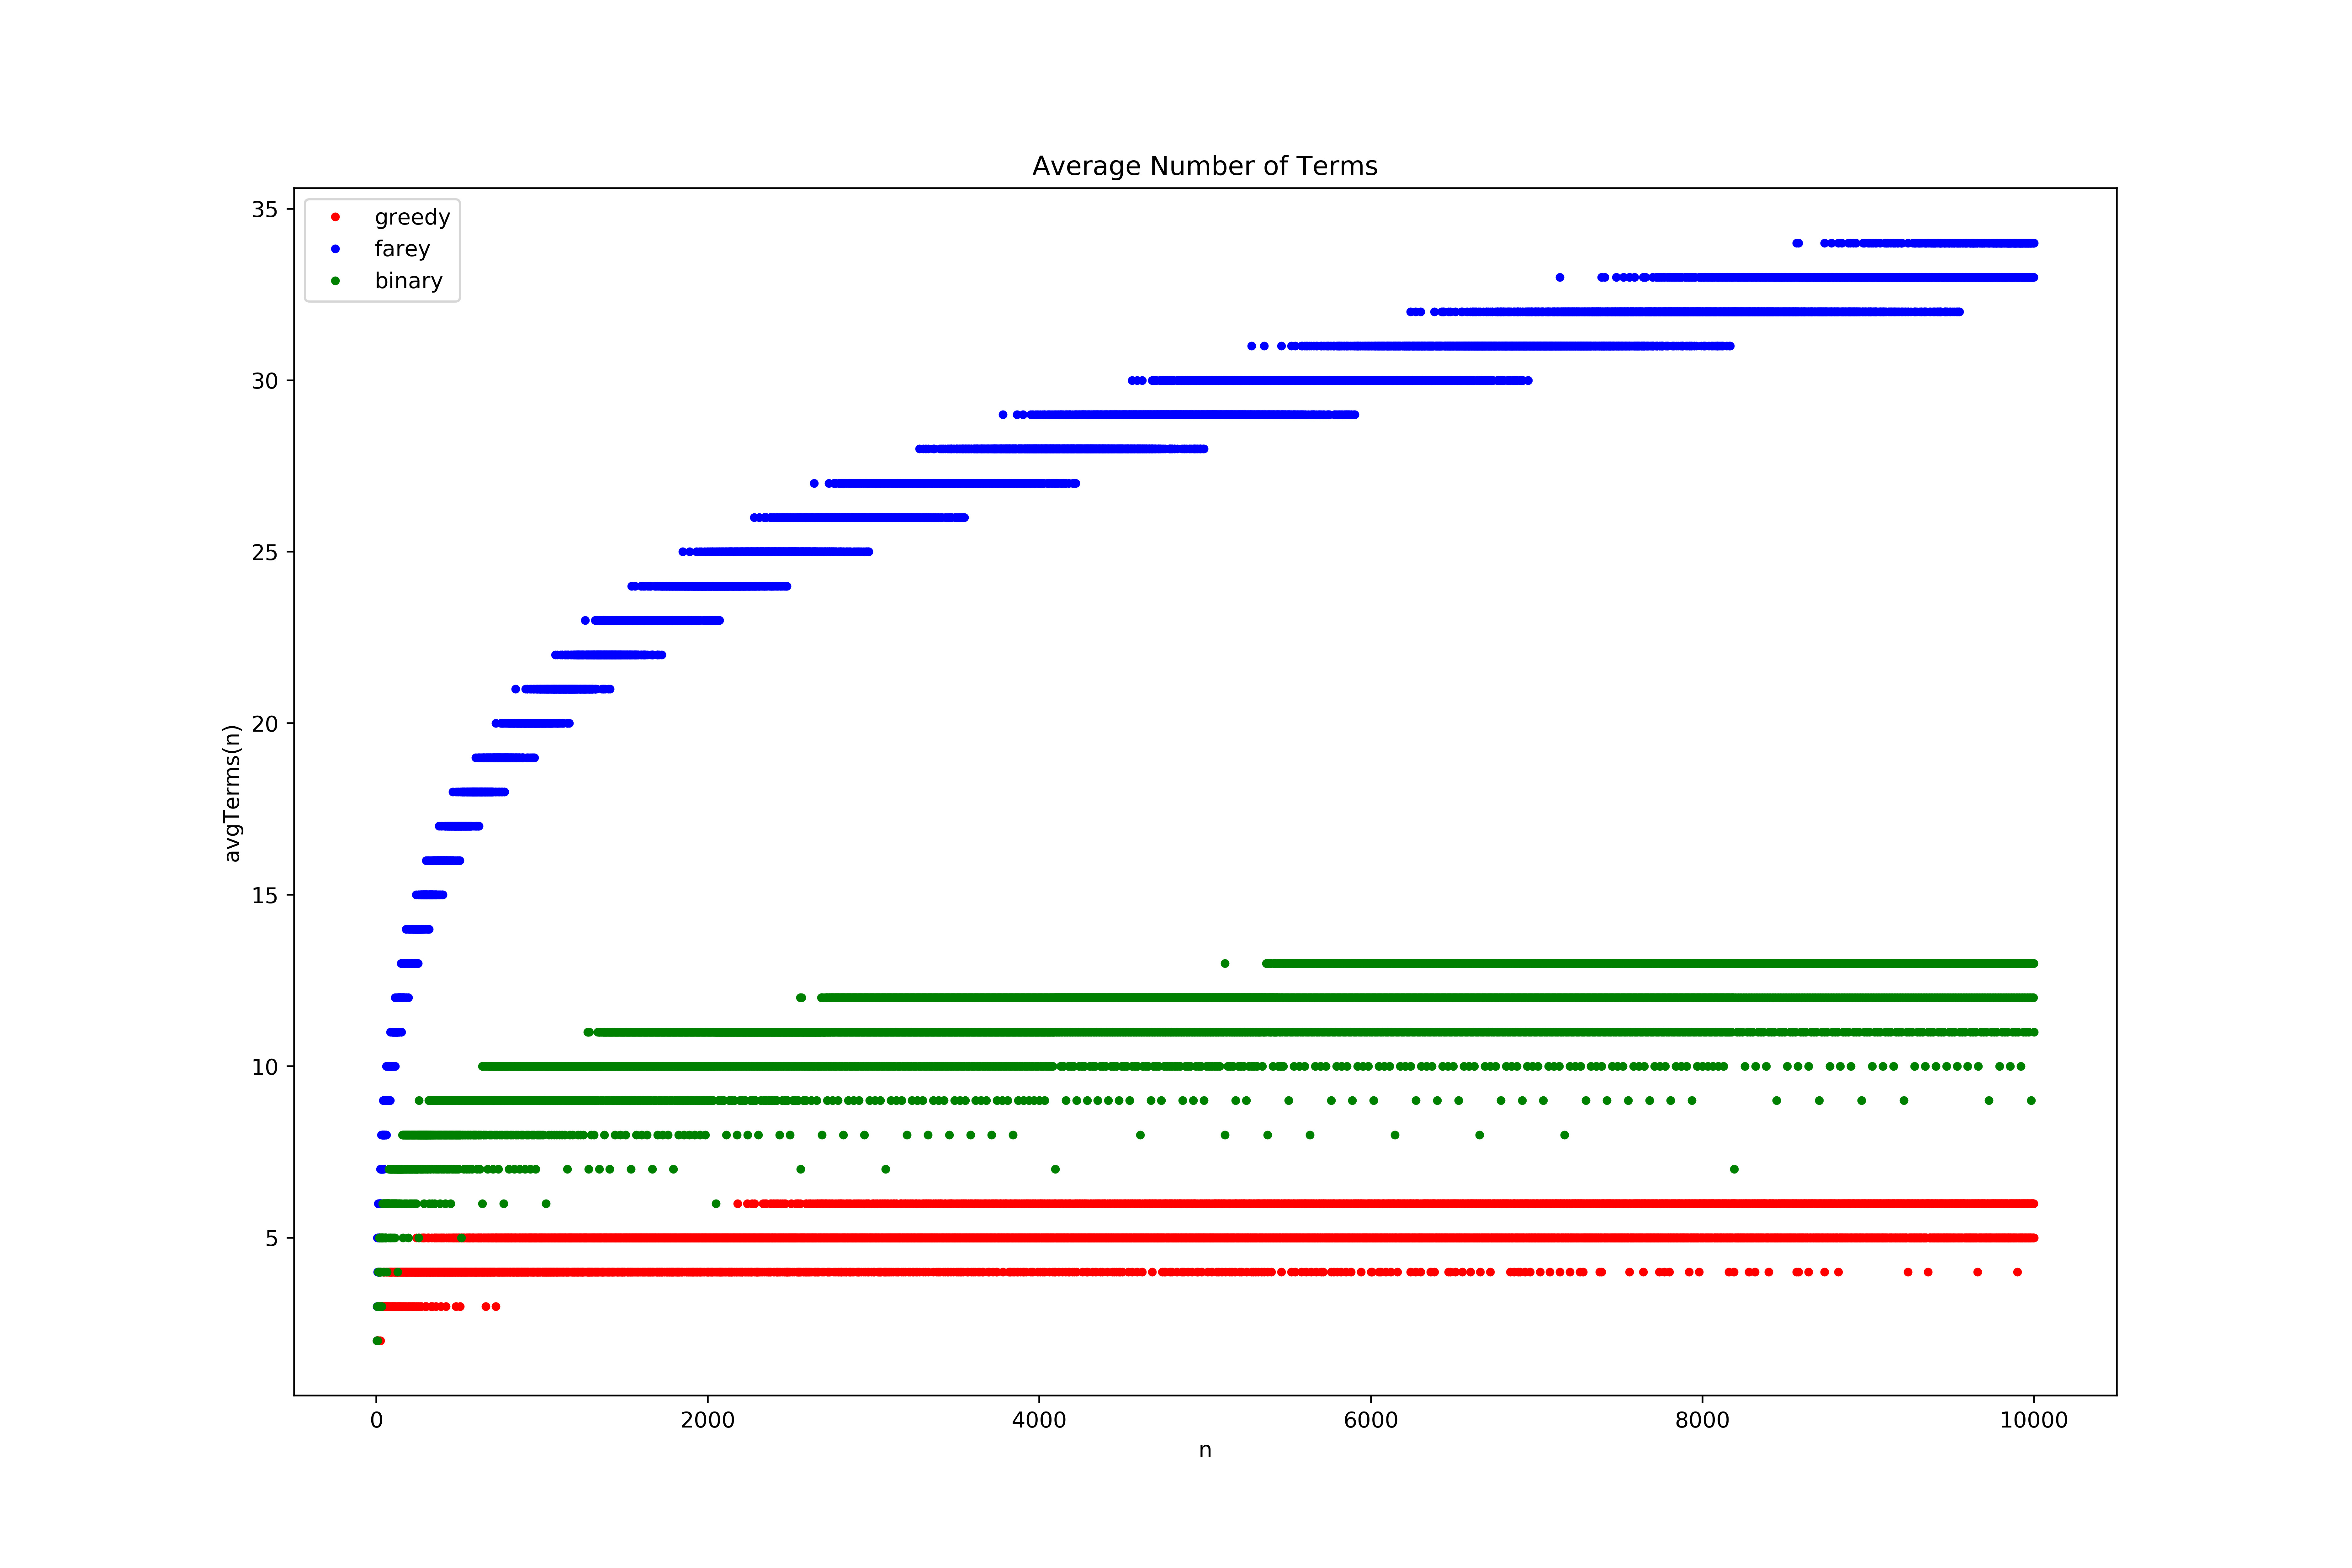
\includegraphics[width=\textwidth]{images/avgTerms.png}
\end{figure}
}{}

\subsubsection{Minimale Anzahl der Terme}
Bezüglich der minimalen Anzahl der produzierten Terme liefert der Greedy-Algorithmus für alle $n$ den gleichen Wert $minTerms_{greedy}(n) = 2$, was jeweils am Ergebnis des Bruchs $\frac{2}{n}$, liegt, welches immer 2 Summanden hat, da der Greedy-Algorithmus jeweils nach der Rechenvorschrift aus Satz \ref{satz:two/n} vorgeht, die wir später noch betrachten werden. Der Farey-Folgen-Algorithmus liefert ständig zwischen $2$ und $3$ alternierende Werte, wobei $n=6$ eine Ausnahme liefert mit $minTerms_{farey}(6) = 5$, da aufgrund der vielen Kürzungen im Datensatz für $n=6$ nur $\frac{5}{6}$ betrachtet wird, welcher in der Farey-Zerlegung 5 Terme benötigt. Beim Binär-Algorithmus erreichen die meisten Tests ein Minimum von 2 Termen pro Datensatz, in ca. $0,7\%$ der Fälle liegt das Minimum jedoch bei 3 Termen. Ein besonderer Zusammenhang zwischen solchen Datensätzen wurde nicht gefunden.

%\ifthenelse{\boolean{printGraphics}}{
%\begin{figure}[H]
%	\label{img:minTerms}
%	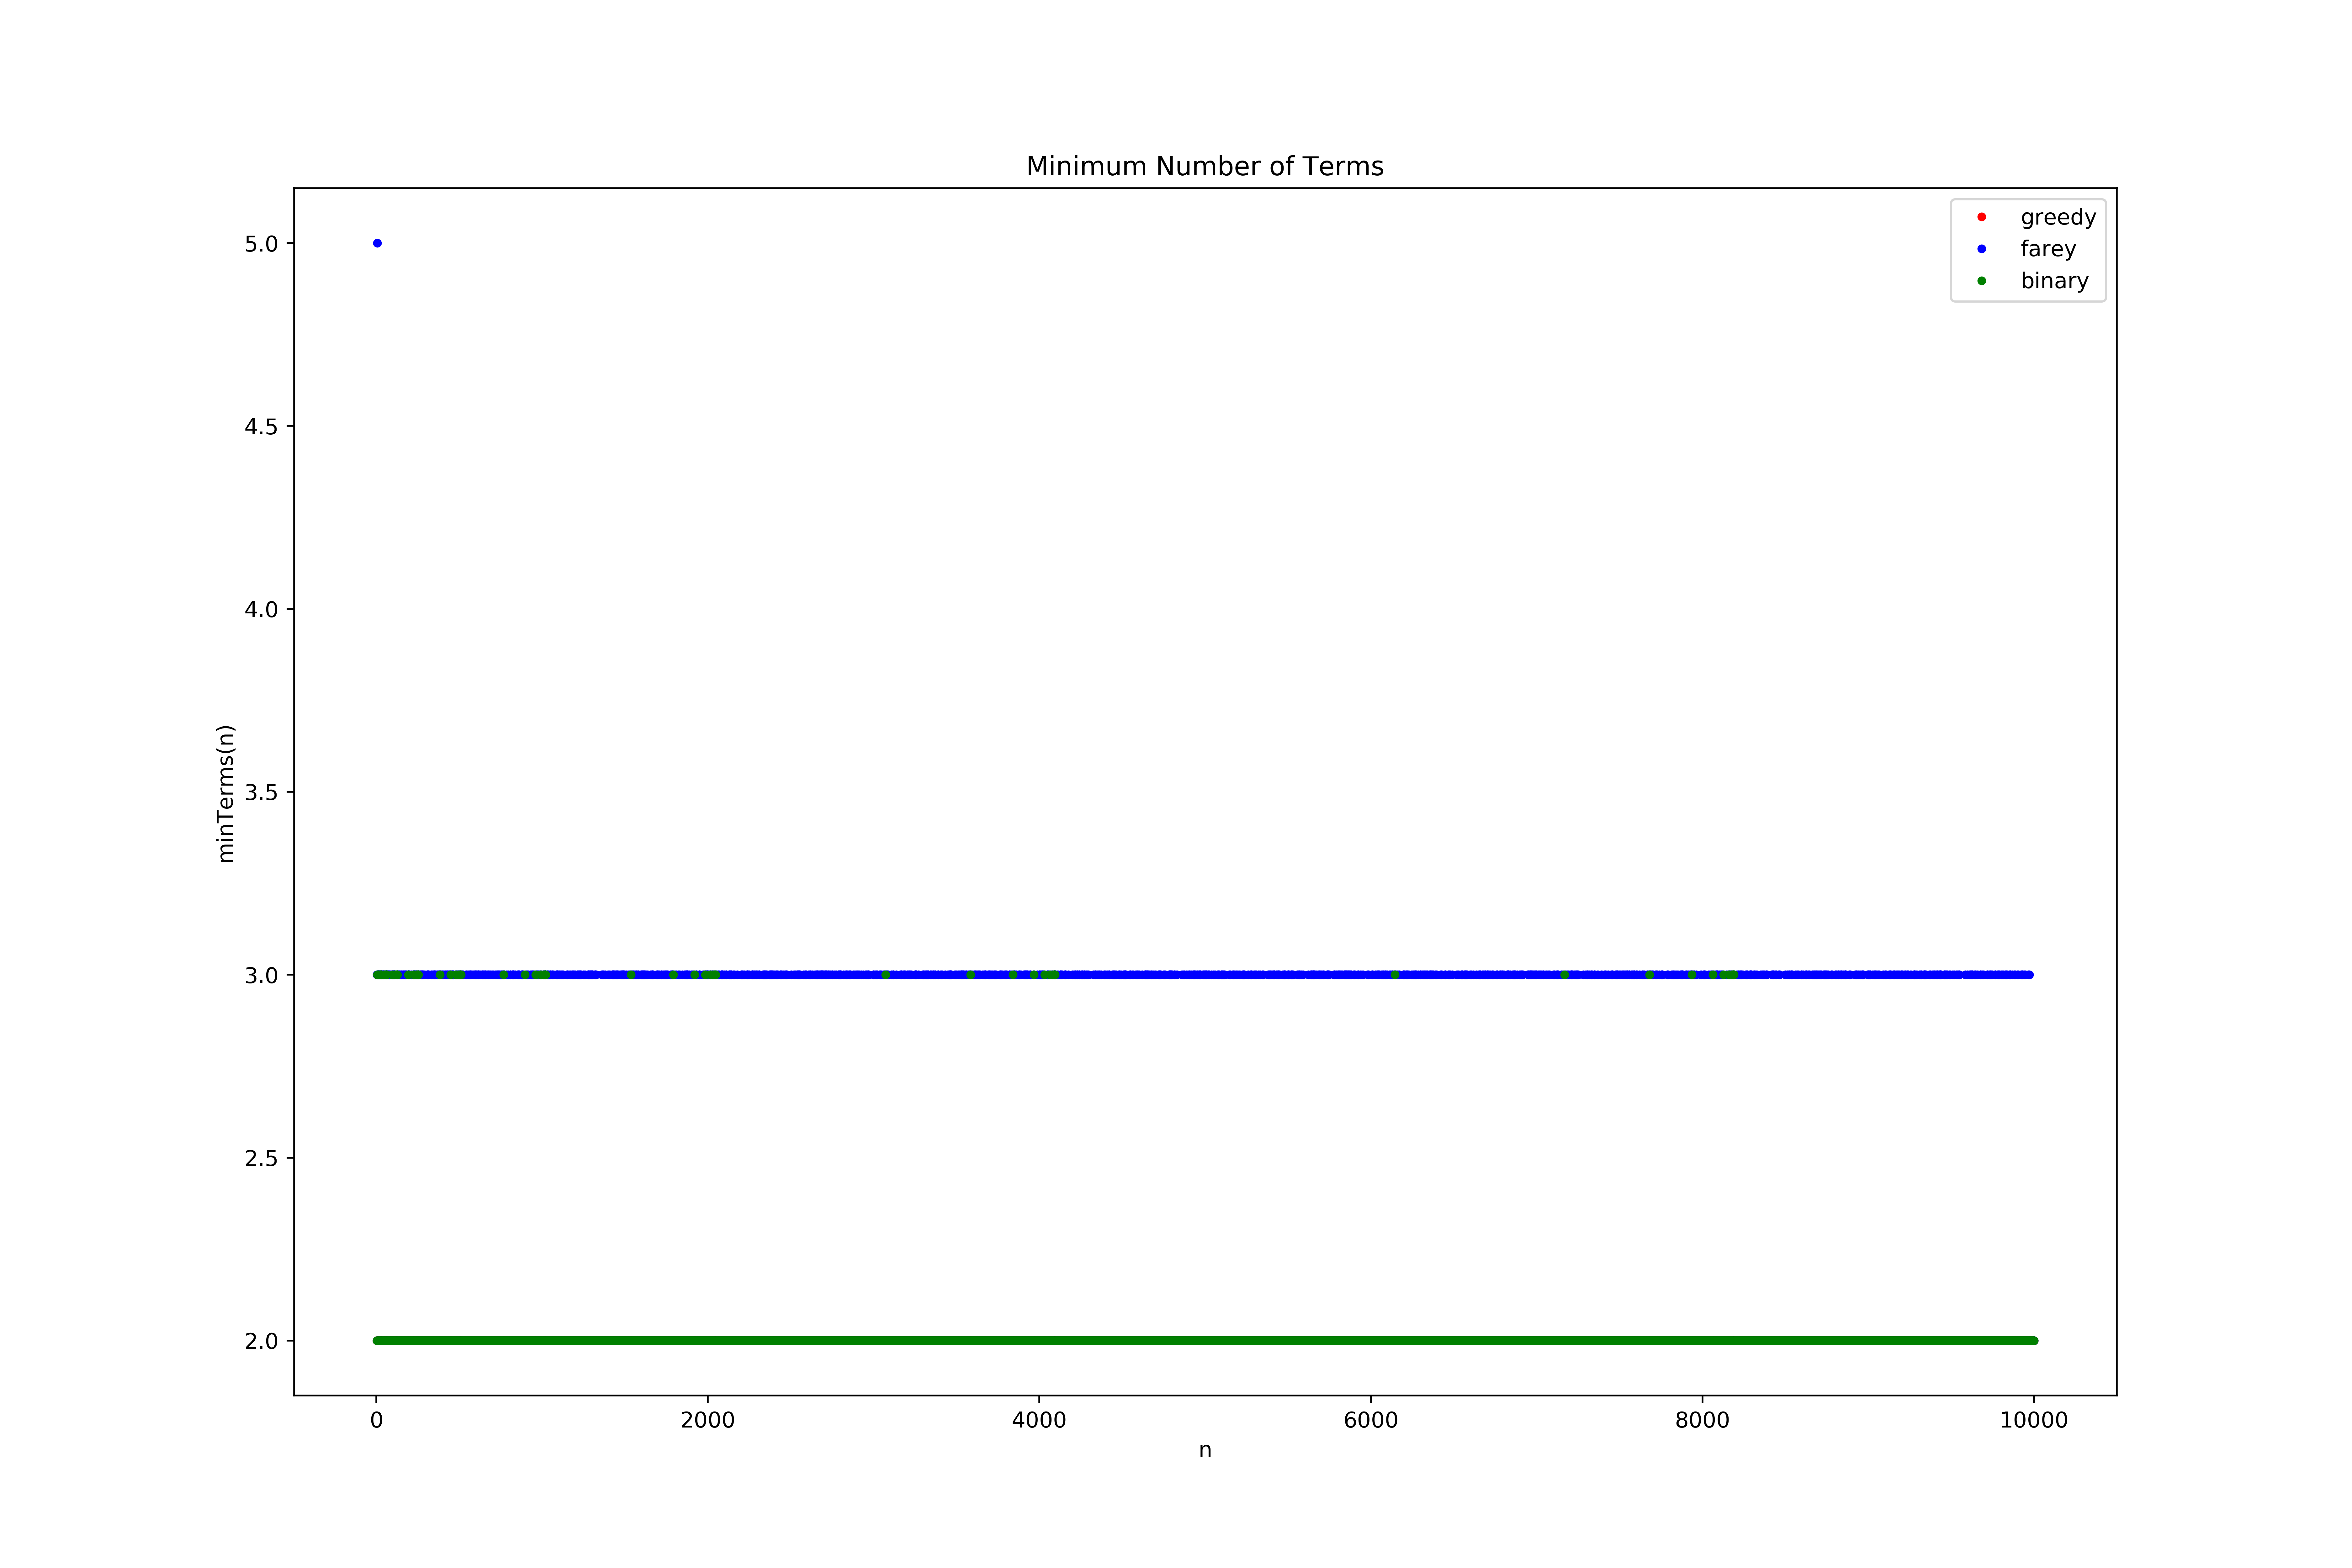
\includegraphics[width=\textwidth]{images/minTerms.png}
%\end{figure}
%}{}


\subsubsection{Maximale Anzahl der Terme}
 Der Greedy-Algorithmus pendelt sich für $3.000 \leq n \leq 10.000$ bei Werten von $7 \leq maxTerms_{greedy}(n) \leq 16$ ein, während der Binäralgorithmus sich im Bereich $2000 \leq n \leq 10.000$ mit Werten von $15 \leq maxTerms_{binary}(n) \leq 22$ mit vernachlässigbar wenig Abweichungen einpendelt. Stiegen die Nenner weiter, wäre das Wachstum nicht beschränkt und würde sich logarithmisch fortsetzen. Für den Farey-Folgen-Algorithmus hingegen gilt ein lineares Wachstum:
$$maxTerms_{farey}(n) = n + 1, \, \forall n$$
für alle getesteten Datensätze. 
\ifthenelse{\boolean{printGraphics}}{
\begin{figure}[H]
	\caption{Maximale Anzahl der Terme im Datensatz für jedes $n$}
	\label{img:maxTerms}
	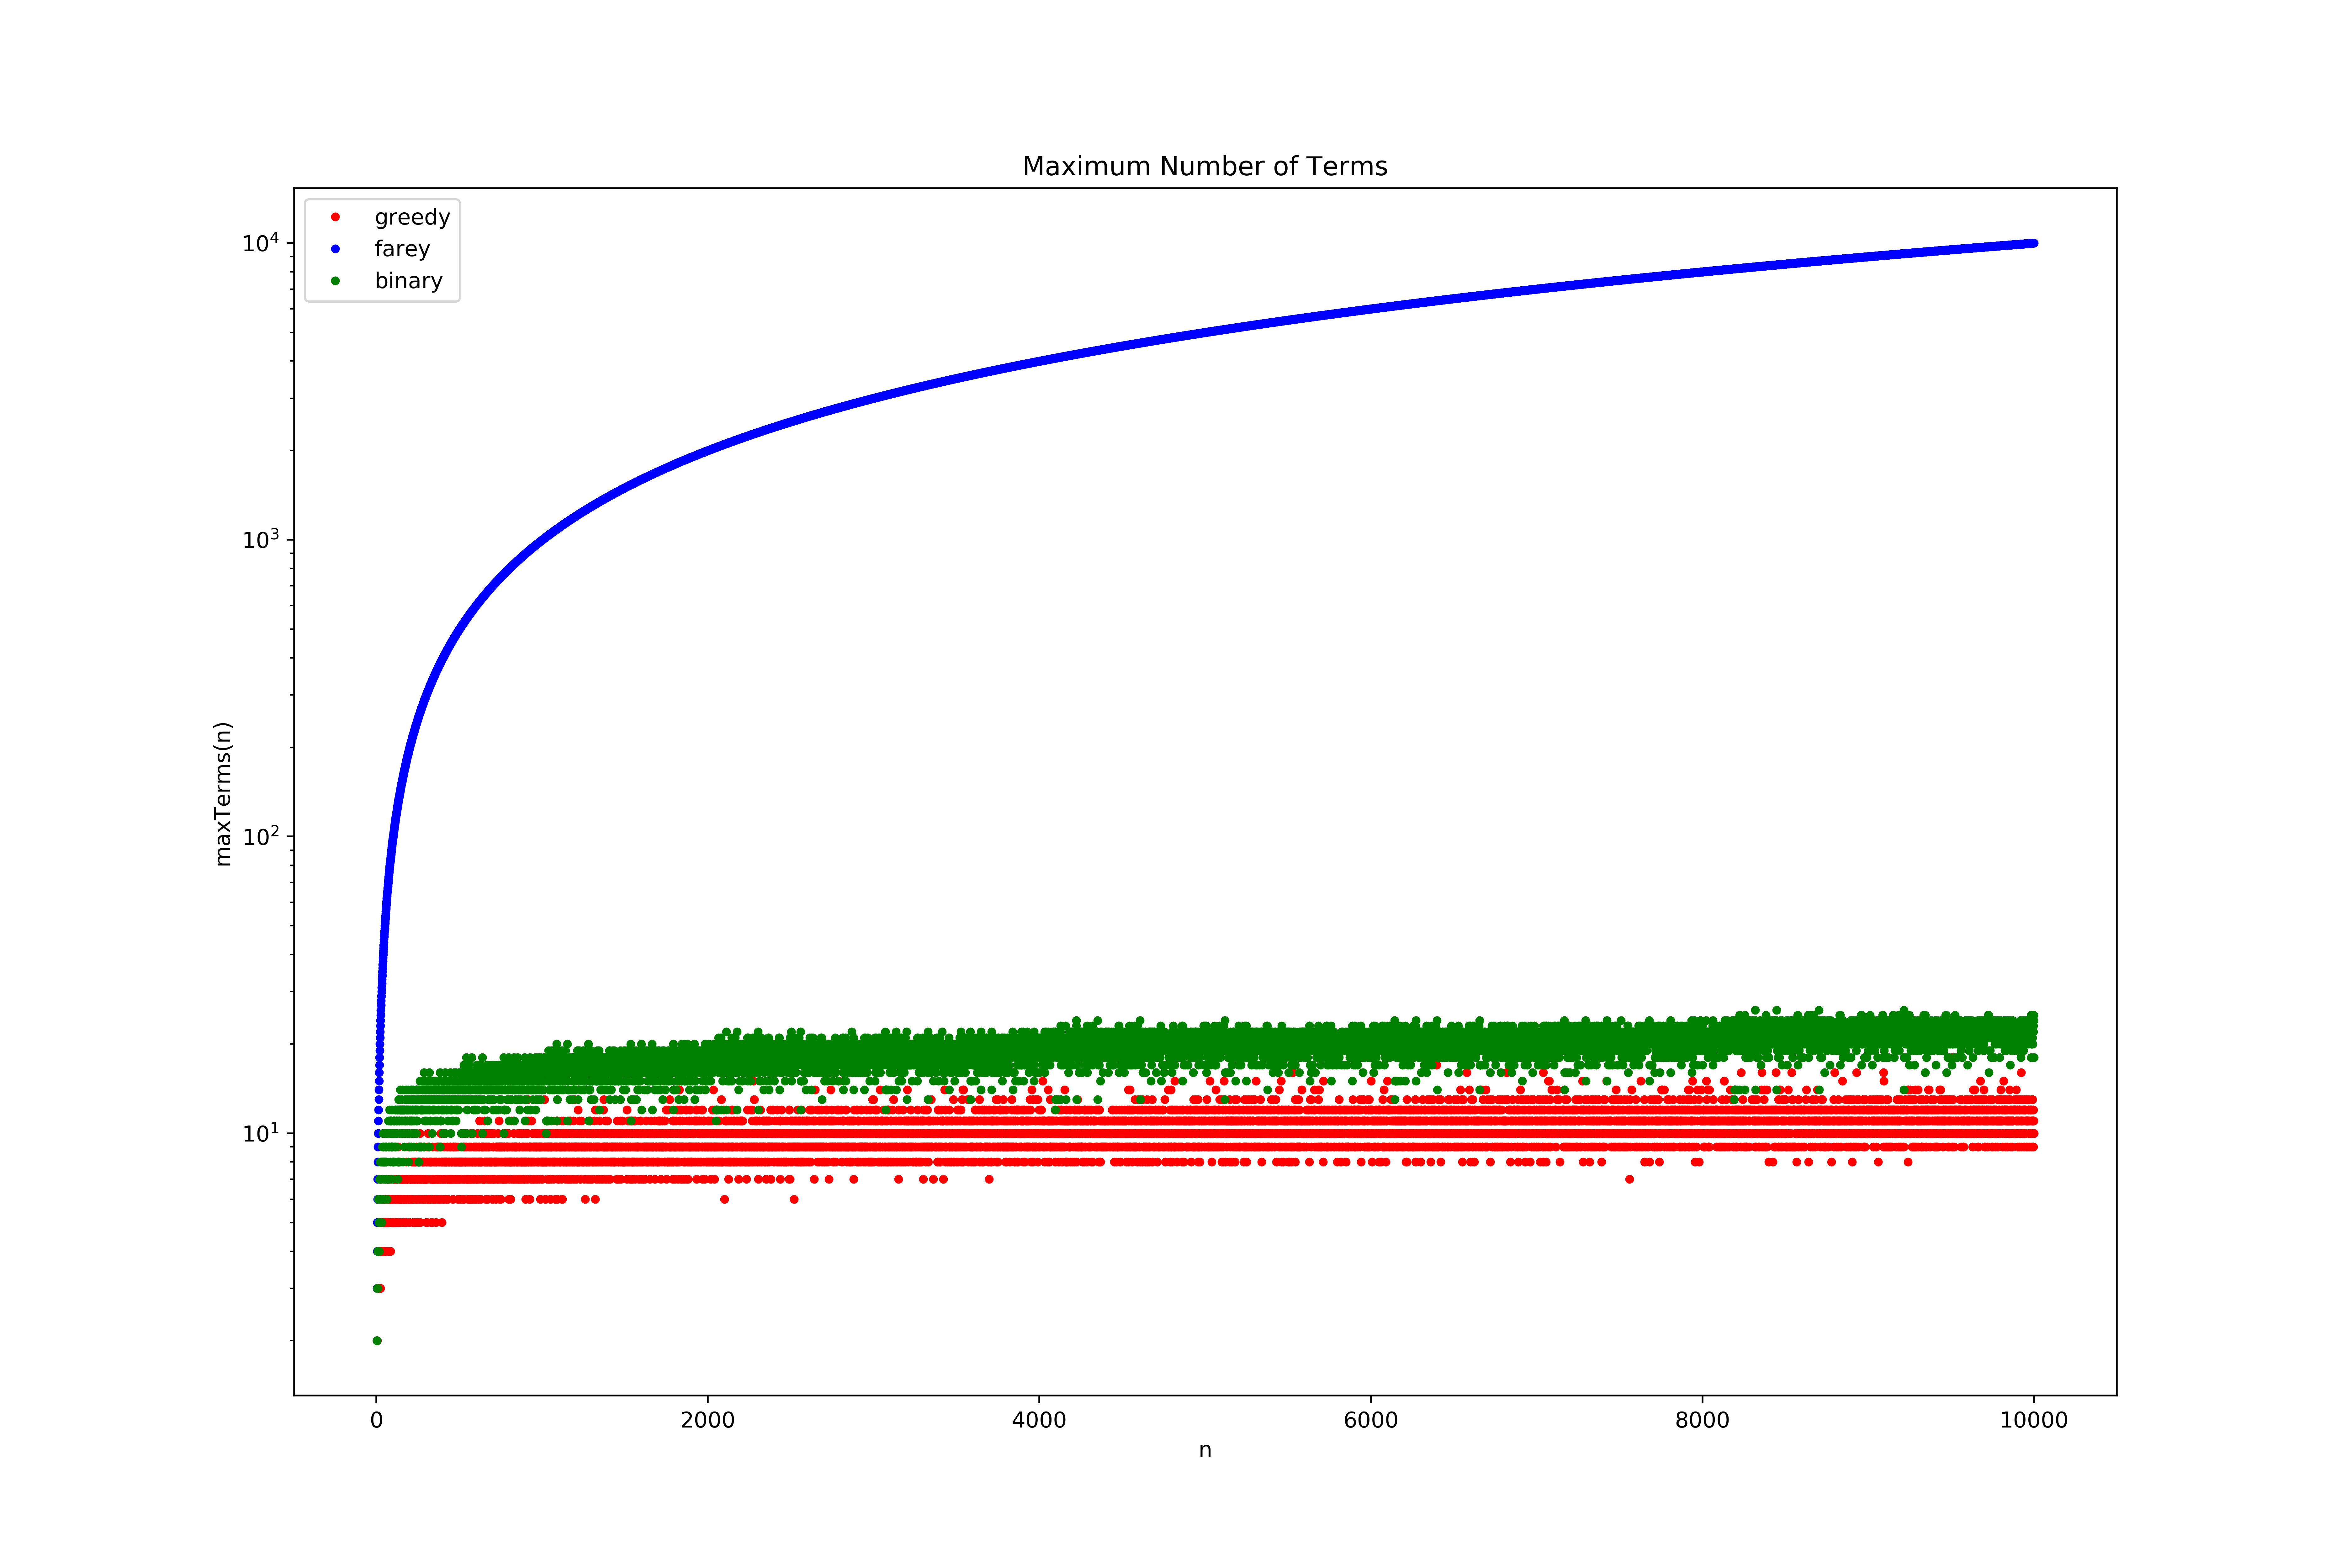
\includegraphics[width=\textwidth]{images/maxTerms.png}
\end{figure}
}{}


\subsubsection{Minimum der größten Nenner}
Sei $u \in \Q$ und bezeichne im Folgenden den Anstieg der linearen Funktion $f(n)=u \cdot n$.\\
Bezüglich des Minimums der größten Nenner zeigen alle Algorithmen klares lineares Wachstum, allerdings in sehr unterschiedlichen Ausprägungen.\\ 
Die Datenpunkte für den Binäralgorithmus ergeben zwei Geraden, eine für alle Werte, bei denen $n$ Zweierpotenz ist, und eine für alle anderen Werte. Das liegt am Sonderfall 2 aus Algorithmus \ref{algo:binary}, der Brüche mit Nennern, die Zweierpotenzen sind, gesondert behandelt und dadurch kleinere Nenner in der Zerlegung produziert. Das lineare Wachstum der beiden Geraden entsteht durch das wachsende $q$ in der Gleichung $\frac{p}{q} = \frac{s}{N_k} + \frac{r}{qN_k}$. Die Gerade der Zweierpotenzen wächst dabei mit Anstieg $u = 1$, die der nicht-Zweierpotenzen mit Anstieg $u=2$. Eine genauere Betrachtung hierzu findet sich im Abschnitt \ref{subsubsec:ZsmHangBinary}\\
Der Greedy-Algorithmus, dessen Werte bzgl. dieses Kriteriums unterhalb und zum Teil auf denen des Binäralgorithmus liegen, zeigt hingegen mehr als zwei Geraden auf, also entwickeln sich bestimmte Folgen innerhalb der Testreihe dieses Algorithmus gleich, die Folgen sind aber in ihrer Entwicklung voneinander unterscheidbar. Die sich ergebenden Geraden haben einen Anstieg $u \in \left\{ 2, 1, \uf{2}, \uf{4}, ... \right\}$, einige Werte liegen aber auch zwischen diesen Geraden. Genaue Gründe hierfür konnten nicht gefunden werden.\\
Ähnliches zeigt sich beim Farey-Folgen-Algorithmus, für den sich 5 Geraden ergeben, allerdings wird hier die Anzahl der Datenpunkte, die jeweils eine Gerade ergeben, mit wachsendem Anstieg immer weniger. Der Anstieg der Geraden ist dabei immer eine Primzahl, die unterste Datenreihe liegt auf der Funktion $f(x)=2x$, die oberste auf der Funktion $f(x) = 13x$. Eine genauere Untersuchung zeigte, dass für jedes fest gewählte $n$ $minDenom_{farey}(n)$ nur durch genau einen Zähler im Datensatz definiert wird. Die Punkte auf der Funktion $f(x) = 13x$ sind beispielsweise durch die Brüche $\frac{1777}{2310}, \frac{1777}{4620}, \frac{6397}{6930} \text{ und } \frac{6397}{9240}$ entstanden. Die scheinbare Logik dahinter wird bereits durch die darunterliegende Gerade $f(x)=11x$ entkräftet, dort tauchen nur die ersten beiden Brüche $\frac{191}{210} \text{ und } \frac{191}{420}$ mit gleichem Zähler zweier aufeinanderfolgender Datenpunkte auf. Allerdings wiederholen sich einige Zähler mehrfach mit unterschiedlichen Nennern, jedoch ohne jegliches erkennbare Muster. Für die Datenpunkte dieser zweithöchsten Gerade sind zudem die Zähler in etwa gleich oft Primzahlen wie nicht Primzahlen. Die Anzahl der Datenpunkte, die auf einer der Geraden liegen, steigt mit sinkendem Anstieg etwa quadratisch.
\ifthenelse{\boolean{printGraphics}}{
\begin{figure}[H]
	\caption{Minimum des größten Nenners im Datensatz für jedes $n$}
	\label{img:minDenom}
	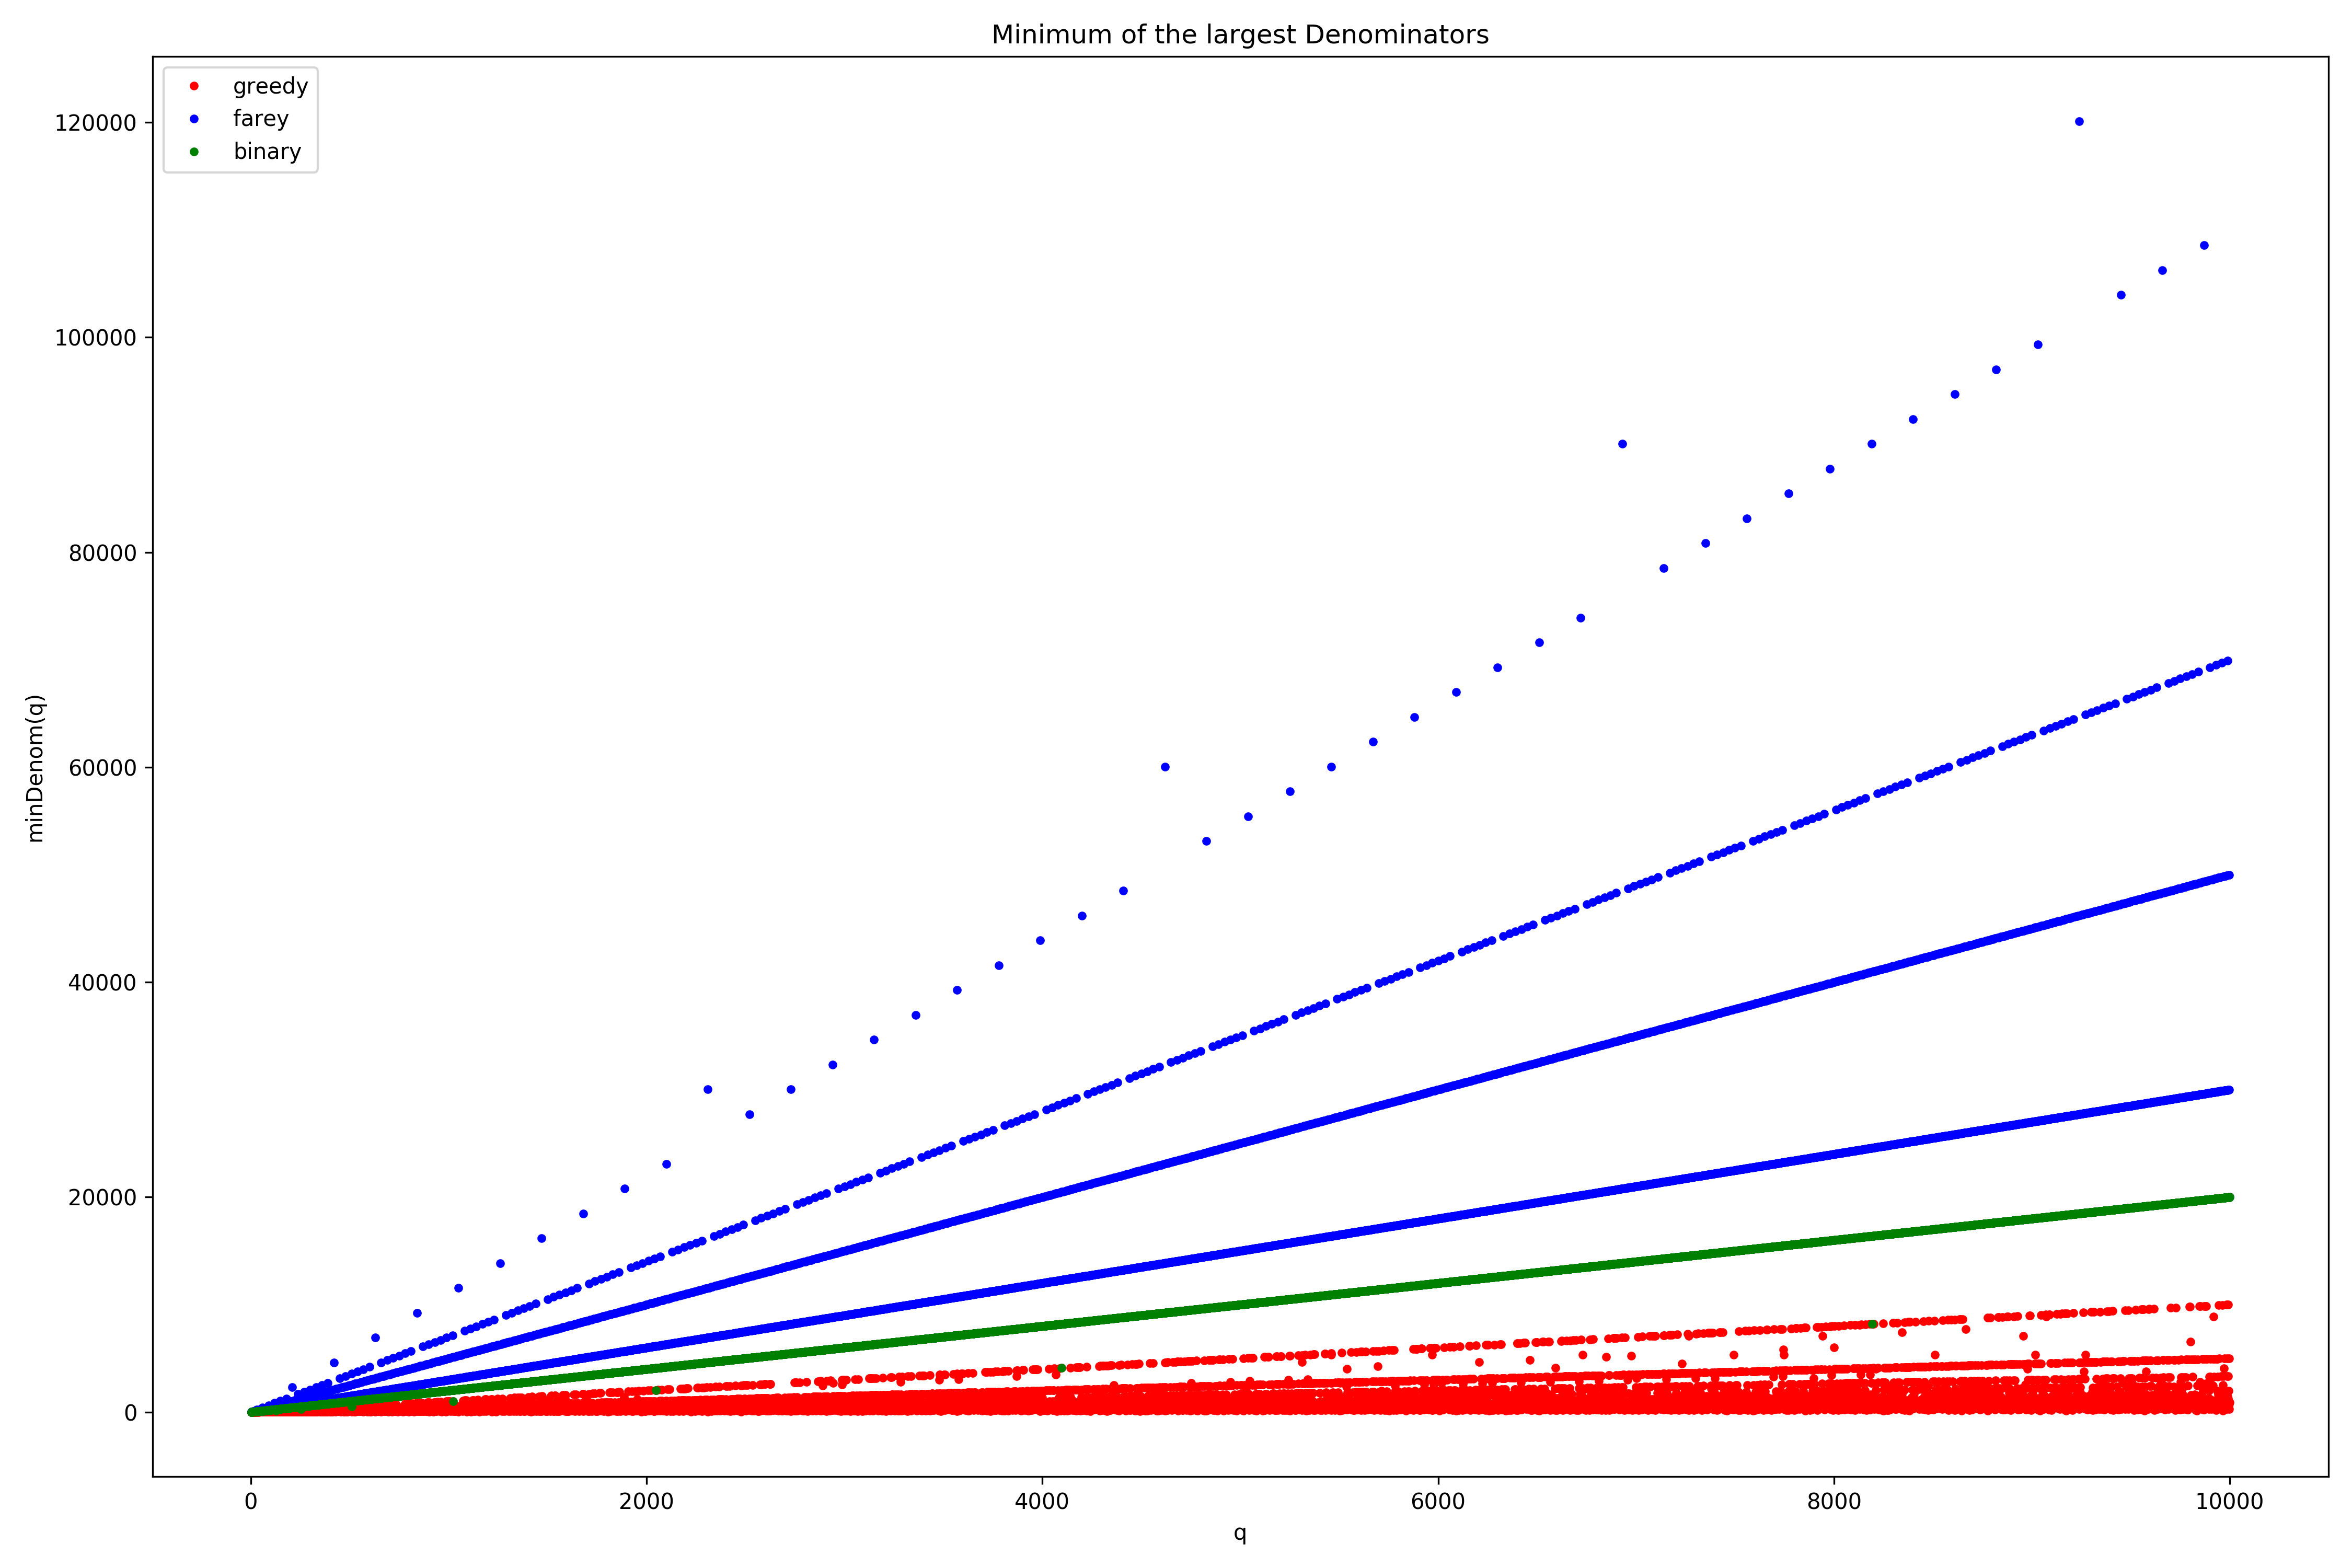
\includegraphics[width=\textwidth]{images/minDenom.png}
\end{figure}
}{}


\subsubsection{Maximum der größten Nenner}
Dieses Kriterium ist jenes, in welchem sich die Algorithmen wohl am stärksten voneinander unterscheiden. Während sich die Werte von Binär- und Farey-Folgen-Algorithmus unter $10^{19}$ halten, streuen sich die Werte des Greedy-Algorithmus von $maxDenom_{greed}(3) = 2$ bis zu einem Maximum von $maxDenom_{greedy}(4967) \approx 7,3378 \times 10^{225.516}$ ohne jegliche erkennbare Regelmäßigkeit. In Abbildung \ref{img:maxDenom} musste auf die Darstellung der 4991 größten Werte des Greedy-Algorithmus verzichtet werden, da diese Werte größer als $10^{250}$ und somit für die Verarbeitung mit \emph{pyplot} zu groß waren.\\
Das Wachstumsverhalten des Binäralgorithmus scheint hier besonders interessant, da sich mehrere Geraden ergeben, die zudem ein sprunghaftes Verhalten aufweisen. Das liegt daran, dass sich der größte Nenner im Binäralgorithmus aus dem Produkt $qN_k$ ergibt, wobei das im Diagramm beschriebene $n=q$ ist. Das $N_k$ ist immer die nächstgrößere Zweierpotenz von $q$, falls $q$ nicht selbst schon eine solche ist. Daher springen die Werte immer bei $q$, falls $q$ Zweierpotenz ist. Das stetig steigende $q$ sorgt zudem für das lineare Wachstum der Geraden, den Anstieg bestimmt $N_k$.\\
Der Farey-Folgen-Algorithmus zeigt für dieses Kriterium ein quadratisches Wachstum auf.

\ifthenelse{\boolean{printGraphics}}{
	\begin{figure}[H]
		\caption{Maximum der größten Nenner pro Datensatz, links: mit Graph für den Greedy-Algorithmus, rechts: ohne selbigen}
		\label{img:maxDenom}
		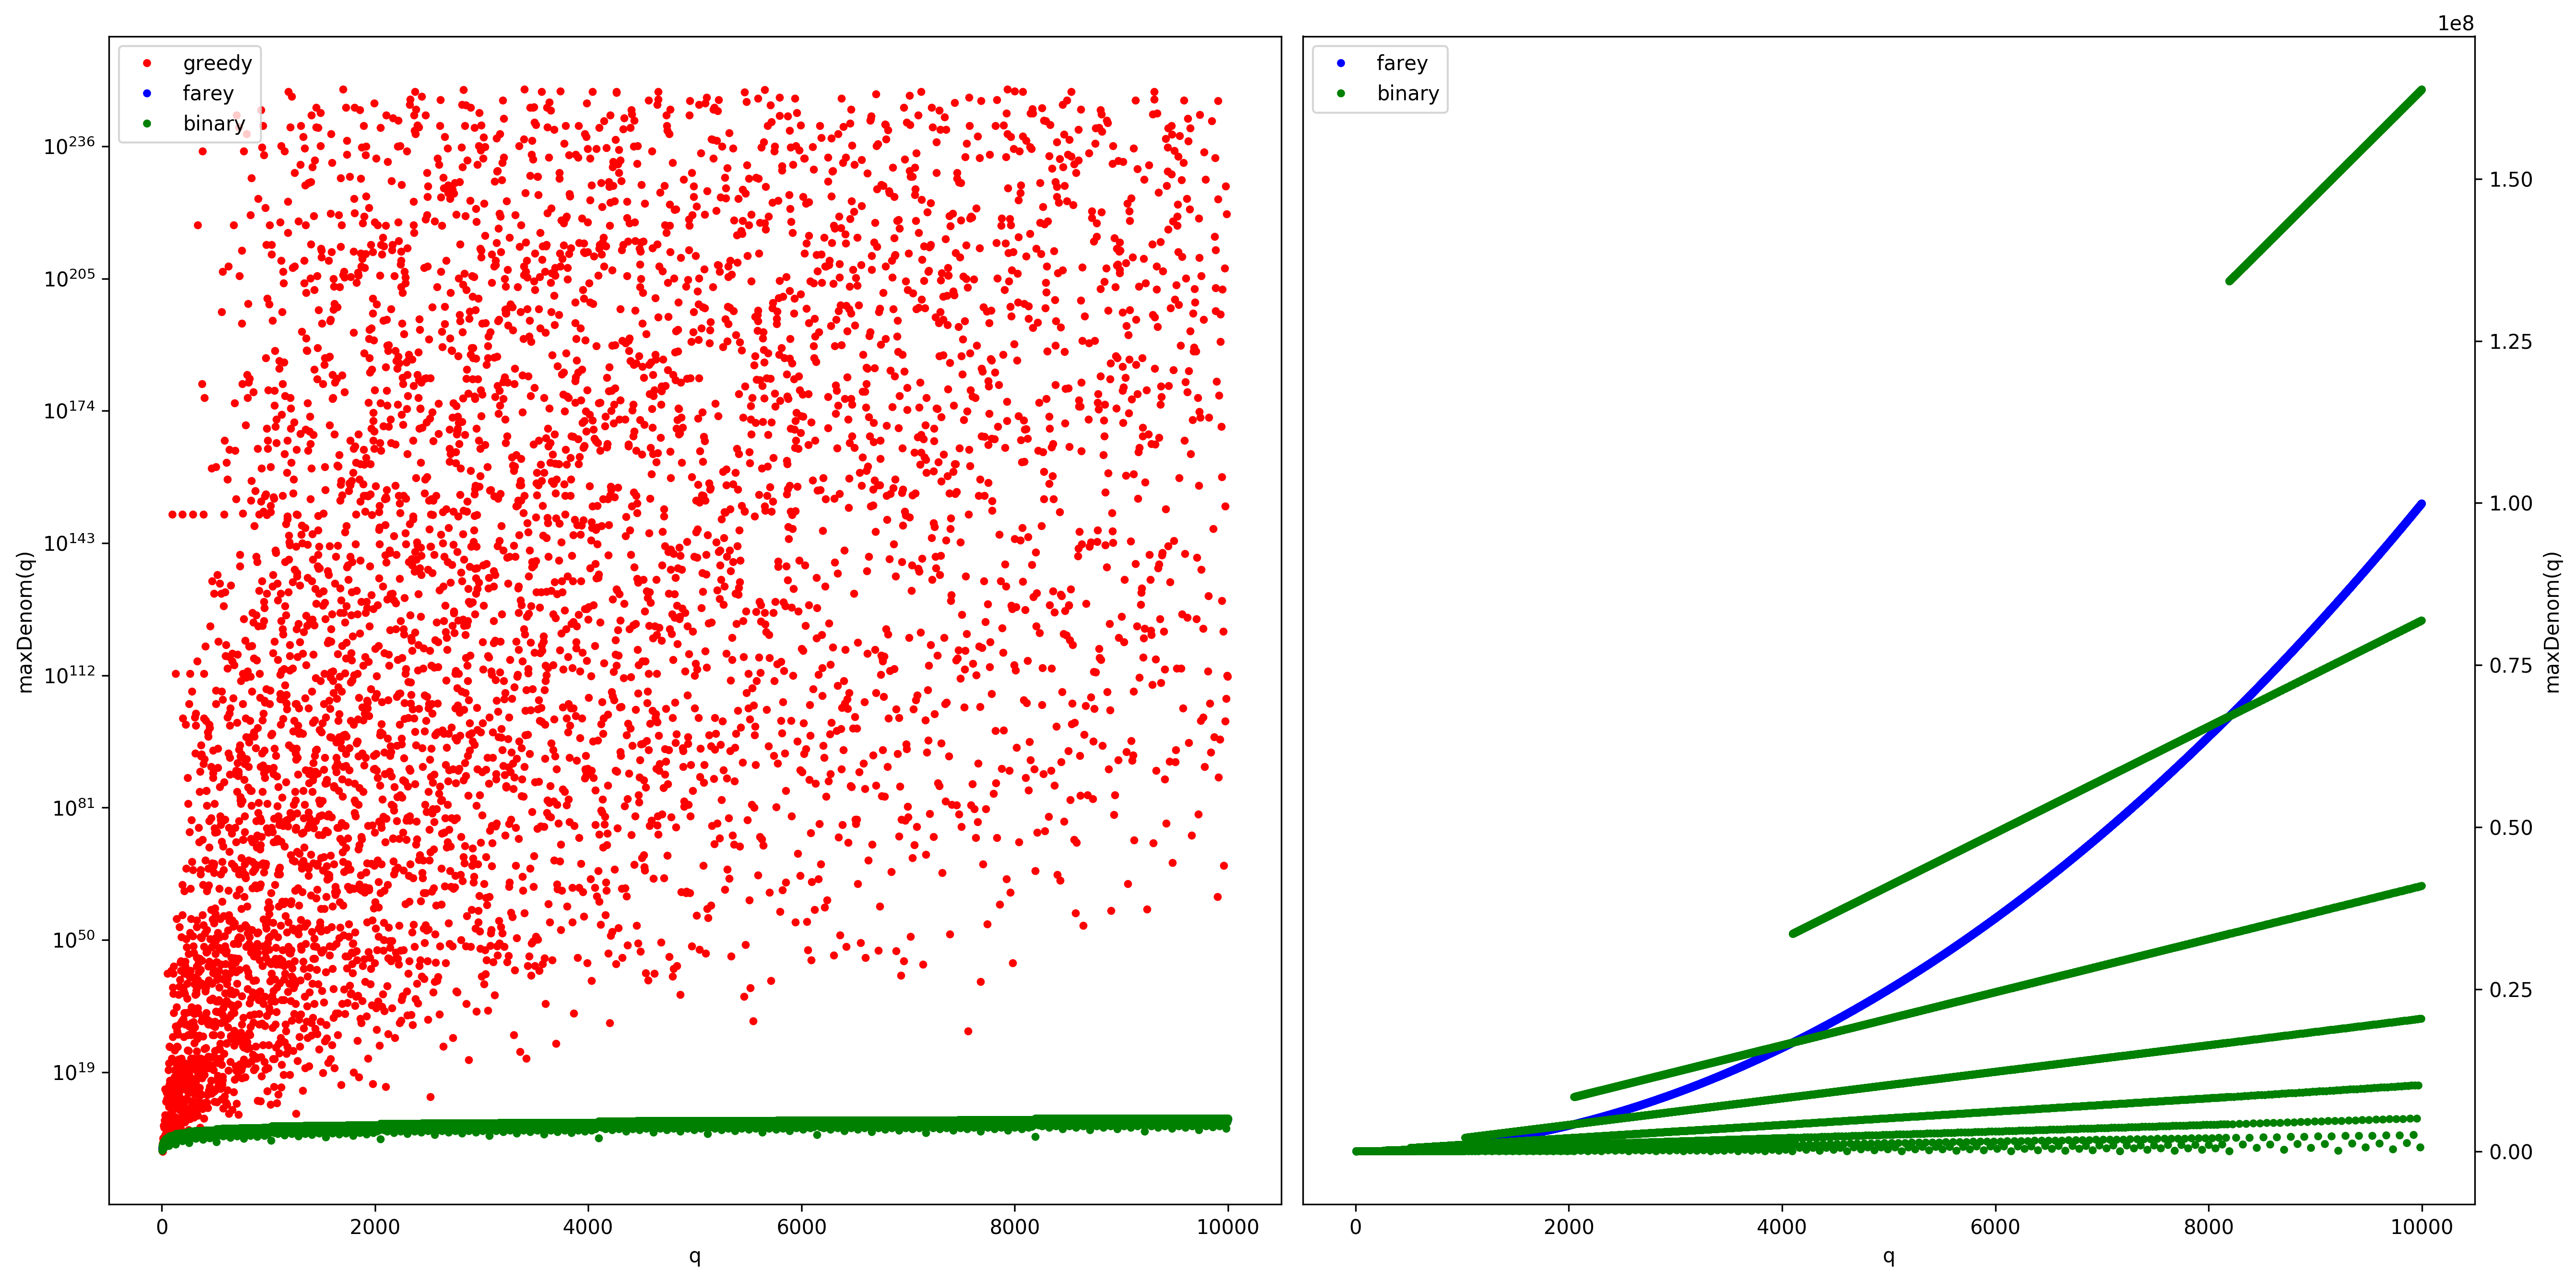
\includegraphics[width=\textwidth]{images/maxDenom2in1.png}
	\end{figure}
}{}

\subsubsection{Zusammenhang innerhalb des Binäralgorithmus}\label{subsubsec:ZsmHangBinary}
Im Binary-Algorithmus konnte eine einfache, aber aussagekräftige Korrelation zwischen $n$ und $minDenom(n)$ nachgewiesen werden:
\begin{equation*}
	minDenom_{binary}(n) = 
	\begin{cases}
		n & \text{falls n Zweierpotenz ist} \\
		2n & \text{sonst.}
	\end{cases}
\end{equation*}
Begründen lässt sich das mit der Zerlegung des Zählers im Schritt 2 des Algorithmus \ref{algo:binary}, für den bei ungeraden Nennern in der Zerlegung immer eine 1 vorkommt, die nicht mit dem Zähler $n$ gekürzt werden kann und somit den kleinsten Bruch $\uf{n}$ bildet. Falls der Zähler des zu zerlegenden Bruchs gerade ist, kann durch das Kürzen der Nenner nur kleiner werden. Für alle $n$, die Zweierpotenz sind, folgt $minDenom_{binary}(n) = n$. Für den Fall, dass n keine Zweierpotenz ist, entsteht der größte Nenner wieder durch den letzten Term in der Gleichung $\frac{p}{q} = .. = \frac{s}{N_k}+\frac{r}{qN_k}$ aus Schritt 3 des Algorithmus \ref{algo:binary}. Dabei ist in jedem Datensatz einmal das n derart gewählt, dass $\uf{2n} = \frac{r}{nN_k} \gdw r = \frac{N_k}{2}$ gilt. Dadurch ergibt sich der Term $\frac{r}{qN_k} = \uf{2q}$ und es entsteht der Zusammenhang $minDenom_{binary}(n) = 2n$ für alle n, die nicht Zweierpotenz sind.

\subsubsection{Vergleich mit Erwartungswerten}
Zur Überprüfung der in Tabelle \ref{table:Algo_Vergleich} aufgezeigten oberen Schranken sollen diese Werte mit den Ergebnissen der zuvor beschriebenen Testreihen verglichen werden.

\paragraph{Anzahl der Summanden}Die oberen Schranken für sowohl Greedy- als auch Farey-Folgen-Al\-go\-rith\-mus sind hier mit $p$, der Zähler des betrachteten Bruchs, angegeben, beim Binäralgorithmus ist hier nur die Komplexitätsklasse $O(\log q)$ angegeben. Bei Betrachtung der Ergebnisse, die in \ref{img:maxTerms} zusammengefasst sind, zeigen sich der Farey-Folgen- und der Binäralgorithmus mit genau dem erwarteten Verhalten, der Greedy-Algorithmus bleibt sogar weit unter seiner theoretischen Schranke und weist anstelle eines linearen Wachstums nur logarithmisches auf.
\paragraph{Größe der Nenner}Die größtmöglichen Nenner für den Binäralgorithmus werden mit $2(q^2-q)$, für den Farey-Folgen-Algorithmus mit $q(q-1)$, angegeben. Wie an Abbildung \ref{img:maxDenom} zu erkennen ist, halten sowohl Farey-Folgen- wie auch Binäralgorithmus ihre jeweiligen oberen Schranken ein.
Der Greedy-Algorithmus liefert, wie Bleicher und Erdös in ihrem Artikel ''Denominators of Egyptian Fractions''\footnote{engl.: Nenner Ägyptischer Brüche, \cite[S. 157]{BleicherErdoes1976}} schon berichteten, ein exponentielles Wachstum der Nenner, die aufgrund ihrer Größe in Abbildung \ref{img:maxDenom} teilweise nicht dargestellt werden konnten.

\subsection{Zusammenfassung}
Der Greedy-Algorithmus ist der wohl schlechteste der Algorithmen, obwohl er bezüglich der Anzahl der Terme die besten Ergebnisse liefert. Grund dafür ist die Wahl des jeweils größten Nenners, wodurch es zu den extremen numerischen Ausbrüchen der Nenner kommt, die eine effiziente Nutzung des Algorithmus mittels normaler Computersysteme unmöglich macht, da die Standards vieler Programmiersprachen solch große \bzw kleine Zahlen nicht unterstützen. Durch die großen Schwankungen zwischen den Werten des Greedy-Algorithmus ist dieser zudem sehr unvorhersehbar. Obwohl er in den meisten Fällen durchaus brauchbare Ergebnisse liefert, ist nicht vorhersagbar, wann dies nicht der Fall ist. Im Vergleich dazu tendiert der Farey-Folgen-Algorithmus eher dazu, kleinere Nenner zu erzeugen, benötigt dafür im Durchschnitt aber deutlich mehr Terme. Der Binäralgorithmus bewegt sich in den verglichenen Kriterien meist zwischen den Werten der anderen Algorithmen, aber immer zum geringeren tendierend, von wenigen Punkten der maximalen Nenner abgesehen, in denen er dem Farey-Folgen-Algorithmus leicht unterlegen ist. Zudem hatte er im Vergleich die beste Laufzeit und nach allem Anschein auch den stabilsten Gesamtverlauf. Damit ist diese Berechnungsmethode wohl die gewinnbringendste, da sie mit relativ wenig Aufwand durchaus brauchbare Zerlegungen gemeiner in Ägyptische Brüche erzeugt.
\clearpage
\section[Theoretische Schranken]{Theoretische Schranken für die maximale Anzahl der Stammbrüche}\label{sec:theorie}
Nachdem untersucht wurde, was in der Praxis mit ausgewählten Methoden erreicht werden kann, soll nun das Licht auf einen weiteren sehr interessanten Aspekt Ägyptischer Brüche gelenkt werden, nämlich den Dingen, die theoretische herleitbare Schranken haben. Vor allem im 20. Jahrhundert wurde von zahlreichen Mathematikern an dem Problem, solche theoretischen Grenzen zu finden und zu beweisen, gearbeitet, unter ihnen Bleicher, Erdös, Graham und andere \cite[S.87 ff]{Guy1981}.

\begin{satz}\label{satz:two/n}
	Sei $n \in \N$ ungerade. $\frac{2}{n}$ lässt sich für jedes $n$ als Summe zweier Stammbrüche notieren, nämlich:
	$$\frac{2}{n} = \uf{\lceil \frac{n}{2} \rceil} + \uf{n \cdot \lceil \frac{n}{2} \rceil}.$$
\end{satz}
\begin{bew}
	Sei $m \in \N$ so gewählt, dass $n=2m+1$. Es folgt:
	\begin{eqnarray*}
		\uf{\lceil \frac{n}{2} \rceil} + \uf{n \cdot \lceil \frac{n}{2} \rceil} & = & \uf{m+1} + \uf{(2m+1)(m+1)}\\
		& = & \frac{2m+1}{(2m+1)(m+1)} + \frac{1}{(2m+1)(m+1)}\\
		& = & \frac{2m+2}{(2m+1)(m+1)}\\
		& = & \frac{2(m+1)}{(2m+1)(m+1)}\\
		& = & \frac{2}{2m+1}\\
		& = & \frac{2}{n}.
	\end{eqnarray*}
\end{bew}

Da der Term $\uf{\lceil \frac{n}{2} \rceil}$ genau dem größten Stammbruch entspricht, der kleiner als $\frac{2}{n}$ ist, liefert der Greedy-Algorithmus hier für alle $\frac{2}{n}$ das gleiche Ergebnis wie die Rechenvorschrift aus Satz \ref{satz:two/n}. Damit lässt sich auch sofort eine weiterer Satz aufstellen, diesmal für $\frac{3}{n}$.

\begin{satz}
	Für jedes beliebige $n \in \N$ lässt sich $\frac{3}{n}$ als Summe von höchstens 3 Stammbrüchen schreiben.
\end{satz}
\begin{bew}
	Es gilt
	$$\frac{3}{n} = \uf{n} + \frac{2}{n}.$$
	Falls $n$ gerade ist, reichen sogar nur zwei Stammbrüche, denn dann kann $\frac{2}{n} = \uf{\frac{n}{2}}$ geschrieben werden; anderenfalls wird $\frac{2}{n}$ wie nach Satz \ref{satz:two/n} zerlegt und es ergeben sich genau drei Stammbrüche:
	$$\frac{3}{n} = \uf{n} + \uf{\lceil \frac{n}{2} \rceil} + \uf{n \cdot \lceil \frac{n}{2} \rceil}.$$
\end{bew}

Bleicher und Erdös vermuteten, dass für alle $n \in \N$ der Bruch $\frac{4}{n}$ in höchstens 3 Stammbrüche zerlegt werden kann, was nicht formal bewiesen, aber von Nicola Franceschine zumindest für $n < 10^8$ gezeigt wurde. Die gleiche Vermutung für $\frac{5}{n}$ wurde durch W. Sierpiński aufgestellt, zunächst durch G. Palamá für alle $n < 922.321$ gezeigt und später durch Stewart auf alle $n < 1.057.438.801$, $n \not\equiv 1\, (\text{mod } 278.460)$ erweitert.
Schinzel bewies zudem, dass der Ausdruck
$$\frac{4}{at+b} = \uf{x(t)} + \uf{y(t)} + \uf{z(t)}$$
für Polynome $x(t), y(t)$ und $z(t)$ mit ganzzahligen Koeffizienten genau dann gilt, wenn $b$ nicht quadratischer Rest modulo $a$ ist. \cite[S. 88]{Guy1981}
\todo[inline]{mehr Theorie!!}
Bereits das vergleichsweise einfache Beispiel $\frac{4}{n}$, für welches noch immer nicht klar ist, ob es sich für alle $n \in \N$ durch höchstens 3 Stammbrüche als Ägyptischer Bruch darstellen lässt, zeigt auf, wie viel in diesem Bereich der Mathematik noch unbekannt ist. Das Problemfeld der Ägyptischen Brüche, das vor knapp 4000 Jahren aufgeworfen wurde, stellt auch die heutigen Mathematiker noch vor viele ungelöste Aufgaben und Fragen.
\clearpage
% !TEX root = ../document.tex
\section{Anhang}\label{sec:code}

Zur Berechnung der Testreihen aus Abschnitt \ref{sec:Testreihen} wurde ausschließlich der nachfolgend aufgeführte, selbst entwickelte Code in PARI/GP \cite{PARI2018}, Version \emph{2.9.4} umgesetzt.

\subsection{Hilfsfunktionen}
Alle genutzten, nicht in PARI/GP enthaltenen Funktionen sind im Folgenden aufgelistet.

\emph{listsum(list)} berechnet die Summe eines Verbunddatentyps, \bspw einer Liste oder eines Vektors.\\ \emph{listmin(list)} berechnet das Minimum einer Liste, \emph{listmax(list)} das Maximum.
\lstinputlisting[language=gp, firstline=1, lastline=3]{../PARI/algorithms.gp}

\emph{contains(list, element)} durchsucht einen Verbunddatentyp und gibt 1 zurück, falls \emph{element} in \emph{list} enthalten ist, 0 sonst.
\lstinputlisting[language=gp, firstline=89, lastline=96]{../PARI/algorithms.gp}

\emph{reversevecsort(vect)} sortiert \emph{vect} in absteigender Reihenfolge.
\lstinputlisting[language=gp, firstline=98, lastline=104]{../PARI/algorithms.gp}

\emph{FareySeries(order)} berechnet die Farey-Folge der Ordnung \emph{order} und gibt diese als Vektor zurück.
\lstinputlisting[language=gp, firstline=156, lastline=174]{../PARI/algorithms.gp}

\emph{findAdjacent(Fs, fraction)} sucht in der Farey-Folge \emph{Fs} den adjazenten Bruch zu \emph{fraction}, der kleiner ist. Diese Funktion wird seit der Implementierung von \emph{findAdjacentFrel} nicht mehr verwendet und dient seither nur dem Vergleich.
\lstinputlisting[language=gp, firstline=118, lastline=136]{../PARI/algorithms.gp}

\emph{findAdjacentFrel(fract)} berechnet den kleineren der zu \emph{fract} adjazenten Brüche mithilfe des relevanten Teils der Farey-Fogle, wie in Beispiel \ref{bsp:Frel} gezeigt und stellt damit die wesentlich effizientere Alternative zu \emph{findAdjacent(Fs,fraction)} dar.
\lstinputlisting[language=gp, firstline=140, lastline=154]{../PARI/algorithms.gp}

\emph{mediant(frac1, frac2)} berechnet die Mediante zweier Brüche nach Definition \ref{def:mediant}.
\lstinputlisting[language=gp, firstline=138, lastline=138]{../PARI/algorithms.gp}

\emph{findDivisorsOf\_k\_addingup\_n(k,n)} sucht jene Teiler von $k$ heraus, die in ihrer Summe $n$ ergeben.
\lstinputlisting[language=gp, firstline=176, lastline=187]{../PARI/algorithms.gp}

\emph{printEgypFrac(arguments)} nimmt eine Liste mit Argumenten entgegen, die die Funktion dann als Summe aller Elemente als String sowohl ausgibt als auch für eventuelle weitere Verarbeitung zurückgibt.
\lstinputlisting[language=gp, firstline=211, lastline=228]{../PARI/algorithms.gp}


\subsection{PARI/GP Code für den Greedy-Algorithmus}\label{code:greedy}
Die Funktion \emph{fibonacci\_sylvester(fraction, stepsize, start)} berechnet mittels des gleichnamigen Algorithmus die entsprechende Ägyptische Darstellung des Bruchs \emph{fraction}. Das Argument \emph{stepsize} gibt an, um wie viel der Nenner eines Kandidaten bei Bedarf mindestens erhöht wird. $\uf{\text{start}}$ gibt den zuerst untersuchten Kandidaten an. Damit wird die Funktionalität zur Verfügung gestellt, \bspw nur nach Stammbrüchen mit geraden oder ungeraden Nennern zu suchen.\\
Letztendlich ruft der Nutzer aber nur die Stellvertreterfunktionen \emph{greedy}, \emph{greedy\_odd} oder \emph{greedy\_even} auf, die die Hauptfunktion \emph{fibonacci\_sylvester} mit Standardwerten für \emph{stepsize} und \emph{start} nutzen.
\lstinputlisting[language=gp, firstline=5, lastline=38]{../PARI/algorithms.gp}


\subsubsection{Optimierter Greedy-Algorithmus}\label{code:greedy_fast}
Zur Effizienzsteigerung wurde der Greedy-Algorithmus nochmals mit einer wesentlich effizienteren Suche der Nenner umgesetzt, die sich mit dem Namen ''Double \& Add'' beschreiben lässt und dem Prinzip der Ägyptischen Multiplikation aus Abschnitt \ref{subsec:egypMult} entspricht. Die Funktionalität der Suche des größten Stammbruchs $max\{\uf{n}: n \in \N\}$, der kleiner als ein gegebener rationaler Bruch ist, wurde in die Funktion \emph{largestUnitFractionLEQ} ausgelagert. Der Rest des Algorithmus läuft ab wie im Anhang \ref{code:greedy} beschrieben.
\lstinputlisting[language=gp, firstline=40, lastline=87]{../PARI/algorithms.gp}


\subsection{PARI/GP Code für den Farey-Folgen-Algorithmus}\label{code:fareyseries}
Die Implementierung des Farey-Folgen-Algorithmus greift auf eine Dauerschleife zurück, aus der ausgebrochen wird, sobald der Nenner des betrachteten adjazenten Bruchs $1$ ist, was laut Algorithmus \ref{algo:FareySeries} das Abbruchkriterium ist. \emph{adjacent} ist dem Namen entsprechend der aktuelle, kleinere adjazente Bruch zum aktuell untersuchten Bruch \emph{current\_fraction}, \emph{remainder} ist $\uf{qs}$ aus demselben Algorithmus. Wie üblich stellt \emph{result} die Liste der Ergebnissummanden dar.
\lstinputlisting[language=gp, firstline=156, lastline=174]{../PARI/algorithms.gp}

\subsection{PARI/GP Code für den Binäralgorithmus}
\emph{p} und \emph{q} entsprechen Zähler und Nenner des Bruchs \emph{fraction}; \emph{r} und \emph{s} sind die natürlichen Zahlen, aus denen sich gemäß Algorithmus \ref{algo:binary} $qs+r = pN_k$ ergibt. \emph{summands} enthält die Summanden der Zweierpotenzen, die in Summe den Zähler des aktuell betrachteten Bruchs ergeben. \emph{result} ist die Liste der Summanden des Ägyptischen Bruchs.
\lstinputlisting[language=gp, firstline=189, lastline=208]{../PARI/algorithms.gp}

	
	
	
% ######################################
% #                                    #
% #        LITERATURVERZEICHNIS        #
% #                                    #
% ######################################
	\clearpage
	\renewcommand{\refname}{Literaturverzeichnis}
	\bibliography{Bibliography}
	\bibliographystyle{Allgemein/natdin}

% ######################################
% #                                    #
% #             ERKLÄRUNG              #
% #                                    #
% ######################################
	% !TEX root = document.tex
\clearpage
\addsec{Eidesstattliche Erklärung}

% Hinweis: die eidesstattliche Erklärung ist ggfs. an die Richtlinie der IHK anzupassen

Hiermit versichere ich, dass die vorliegende Arbeit selbständig verfasst und keine anderen als die angegebenen Quellen und Hilfsmittel benutzt wurden.\\Ferner habe ich vom Merkblatt über die Verwendung von Bachelor/Masterabschlussarbeiten Kenntnis genommen und räume das einfache Nutzungsrecht an meiner Bachelorarbeit der Universität der Bundeswehr München ein.\\[6ex]

\abgabeOrt, den \abgabeTermin


\rule[-0.2cm]{5.5cm}{0.5pt}

\textsc{\autorName}

	
	
\end{document}